% !TeX root=SBUKThesis-main.tex
\chapter{نتایج و بحث}\label{chap4}

\section{مقدمه}
در این فصل، نتایج حاصل از پیاده‌سازی و ارزیابی مدل پیشنهادی MAGNET برای تشخیص بدافزارهای اندرویدی ارائه می‌شود. مدل MAGNET با بهره‌گیری از داده‌های چندوجهی شامل داده‌های جدولی، گرافی و ترتیبی، و استفاده از معماری‌های پیشرفته نظیر ترنسفورمرها و شبکه‌های عصبی گرافی (\rl{GNN}ها)، طراحی شده است. این مدل با استفاده از مجموعه داده‌های معتبر و با در نظر گرفتن ویژگی‌های مختلف برنامه‌های اندرویدی، آموزش داده شده است.

نتایج به‌دست‌آمده نشان می‌دهد که مدل پیشنهادی با دقت \lr{97.24\%}، \lr{F1 Score} معادل \lr{98.23\%} و AUC برابر با \lr{99.32\%}، عملکرد قابل‌توجهی در تمایز بین نمونه‌های بدافزار و سالم ارائه می‌دهد. هدف این بخش، نمایش یافته‌های خام و بدون تفسیر است تا خواننده بتواند عملکرد مدل را به‌طور شفاف بررسی کند.

در ادامه این فصل، ابتدا معیارهای ارزیابی مورد استفاده معرفی می‌شوند. سپس، نتایج حاصل از آزمایش‌های مختلف با جزئیات کامل ارائه می‌شود. در نهایت، عملکرد مدل پیشنهادی با سایر روش‌های موجود مقایسه می‌شود. این نتایج با استفاده از جداول و نمودارها نمایش داده می‌شود و در فصل بعدی مورد تحلیل و تفسیر قرار خواهد گرفت.

\section{تنظیمات آزمایشی}
برای ارزیابی جامع مدل MAGNET، از مجموعه داده DREBIN \cite{Drebin} استفاده شد که شامل \lr{6,092} نمونه است. این مجموعه داده به دو بخش تقسیم شد: \lr{4,641} نمونه برای آموزش و \lr{1,451} نمونه برای تست (\lr{327} نمونه کلاس \lr{0} و \lr{1,124} نمونه کلاس \lr{1}). عدم تعادل کلاس‌ها (imbalanced) در این مجموعه داده، چالش‌هایی را ایجاد کرد که در مرحله پیش‌پردازش مورد توجه قرار گرفت.

\subsection{ویژگی‌های داده}
داده‌های مورد استفاده شامل دو دسته ویژگی بودند:
\begin{itemize}
    \item \textbf{ویژگی‌های ایستا}: شامل مجوزها، فراخوانی‌های API، مقاصد و نام مؤلفه‌ها
    \item \textbf{ویژگی‌های پویا}: شامل فعالیت شبکه و دسترسی به فایل‌ها
\end{itemize}

پس از پیش‌پردازش، ابعاد ویژگی‌ها به ۴۳۰ ویژگی تنظیم شد و داده‌ها به صورت بردارهای عددی نرمال‌سازی‌شده یا باینری فرمت‌بندی شدند.

\subsection{پیکربندی آزمایش‌ها}
آزمایش‌ها با روش اعتبارسنجی متقاطع ۵-تایی و ۱۰ دوره (epoch) برای هر دسته انجام شدند. بهینه‌سازی ابرپارامترها با دو روش مختلف صورت گرفت:

\begin{itemize}
    \item \textbf{بهینه‌سازی}: با ۴۷۶ آزمایش، که منجر به پیکربندی بهینه زیر شد:
    \begin{itemize}
        \item embedding\_dim = \lr{32}
        \item num\_heads = \lr{4}
        \item num\_layers = \lr{1}
        \item dim\_feedforward = \lr{128}
        \item dropout = \lr{0.2029}
        \item batch\_size = \lr{16}
        \item learning\_rate = \lr{0.00215}
        \item weight\_decay = \lr{0.00107}
        \item num\_epochs = \lr{3}
    \end{itemize}
    
    \item \textbf{Optuna}: با ۱۳ آزمایش، که منجر به پیکربندی بهینه زیر شد:
    \begin{itemize}
        \item embedding\_dim = \lr{64}
        \item num\_heads = \lr{4}
        \item num\_layers = \lr{1}
        \item dim\_feedforward = \lr{128}
        \item dropout = \lr{0.2}
        \item batch\_size = \lr{16}
        \item learning\_rate = \lr{0.0019}
        \item weight\_decay = \lr{0.0011}
        \item num\_epochs = \lr{10}
    \end{itemize}
\end{itemize}

برای بهینه‌سازی از الگوریتم Adam و زمان‌بندی CosineAnnealingWarmRestarts استفاده شد.

\subsection{مدل‌های پایه}
برای مقایسه عملکرد، از مدل‌های پایه زیر استفاده شد:
\begin{itemize}
    \item \textbf{روش‌های یادگیری ماشین کلاسیک}:
    \begin{itemize}
        \item ماشین بردار پشتیبان (\lr{SVM}) با کرنل \lr{RBF}
        \item جنگل تصادفی (\lr{Random Forest}) با \lr{100} درخت
        \item \lr{XGBoost} با \lr{100} درخت و عمق حداکثر \lr{6}
        \item شبکه عصبی مصنوعی (\lr{ANN}) با دو لایه مخفی
    \end{itemize}
    \item \textbf{روش‌های چندوجهی} با دقت \lr{89.2\%} \cite{Alsaleh2023}
    \item \textbf{روش‌های مبتنی بر ترنسفورمر} با دقت \lr{95.8\%} \cite{TransformerMalware}
\end{itemize}

\subsection{محیط اجرا}
تمامی آزمایش‌ها با استفاده از زبان برنامه‌نویسی Python \lr{3.8.5} و کتابخانه‌های زیر اجرا شدند:
\begin{itemize}
    \item PyTorch \lr{1.9.0} برای پیاده‌سازی شبکه‌های عصبی
    \item PyTorch Geometric \lr{1.7.0} برای پردازش داده‌های گرافی
    \item scikit-learn \lr{0.24.2} برای پیش‌پردازش داده‌ها و ارزیابی
    \item NumPy \lr{1.21.2} و Pandas \lr{1.3.3} برای پردازش داده‌ها
\end{itemize}

سخت‌افزار مورد استفاده شامل:
\begin{itemize}
    \item GPU NVIDIA RTX \lr{3090} با \lr{24} گیگابایت VRAM
    \item CPU Intel Xeon E\lr{5}-\lr{2690} v\lr{4} با \lr{32} هسته
    \item \lr{128} گیگابایت RAM
\end{itemize}

\section{معیارهای ارزیابی}
برای سنجش عملکرد مدل MAGNET، معیارهای دقت (Accuracy)، \lr{F1 Score}، Precision، Recall و AUC استفاده شدند. دقت به‌عنوان نسبت نمونه‌های درست طبقه‌بندی‌شده به کل نمونه‌ها تعریف می‌شود:

\begin{equation}
\text{Accuracy} = \frac{\text{TP} + \text{TN}}{\text{TP} + \text{TN} + \text{FP} + \text{FN}}
\end{equation}

که در آن:
\begin{itemize}
    \item TP (True Positive): تعداد بدافزارها که به درستی تشخیص داده شده‌اند
    \item TN (True Negative): تعداد برنامه‌های سالم که به درستی به عنوان سالم تشخیص داده شده‌اند
    \item FP (False Positive): تعداد برنامه‌های سالم که اشتباهاً به عنوان بدافزار تشخیص داده شده‌اند
    \item FN (False Negative): تعداد بدافزارها که اشتباهاً به عنوان برنامه سالم تشخیص داده شده‌اند
\end{itemize}

Precision نسبت نمونه‌های درست مثبت به کل نمونه‌های پیش‌بینی‌شده مثبت است:

\begin{equation}
\text{Precision} = \frac{\text{TP}}{\text{TP} + \text{FP}}
\end{equation}

Recall نسبت نمونه‌های درست مثبت به کل نمونه‌های واقعی مثبت را نشان می‌دهد:

\begin{equation}
\text{Recall} = \frac{\text{TP}}{\text{TP} + \text{FN}}
\end{equation}

F1 Score، معیاری ترکیبی از Precision و Recall، به‌صورت زیر محاسبه می‌شود:

\begin{equation}
\text{F1 Score} = 2 \cdot \frac{\text{Precision} \cdot \text{Recall}}{\text{Precision} + \text{Recall}}
\end{equation}

همچنین، AUC (مساحت زیر منحنی \lr{ROC}) توانایی مدل در تمایز بین کلاس‌های بدافزار و سالم را نشان می‌دهد. در نهایت، ماتریس درهم‌ریختگی \lr{(Confusion Matrix)} برای تحلیل دقیق‌تر پیش‌بینی‌ها استفاده شد.

\section{نتایج کلی مدل MAGNET}
در این بخش، نتایج کلی مدل MAGNET در مراحل مختلف آزمایش گزارش می‌شود. ابتدا نتایج تست روی مجموعه داده DREBIN \cite{Drebin} ارائه می‌شود. مدل MAGNET روی مجموعه تست شامل ۱،۴۵۱ نمونه (۳۲۷ نمونه کلاس ۰ و ۱،۱۲۴ نمونه کلاس ۱) ارزیابی شد. نتایج به‌دست‌آمده شامل \lr{F1 Score} برابر با ۰\lr{.۹۸۲۳}، دقت (Accuracy) برابر با \lr{۰.۹۷۲۴،} Precision برابر با \lr{۰.۹۷۹۶}، Recall برابر با \lr{۰.۹۸۴۹}، AUC برابر با \lr{۰.۹۹۳۲} و مقدار زیان (Loss) برابر با \lr{۰.۱۰۲۲} بود.

\subsection{ماتریس درهم‌ریختگی و عملکرد به تفکیک کلاس}
ماتریس درهم‌ریختگی مدل شامل ۳۰۴ نمونه درست منفی (\lr{TN})، ۲۳ نمونه نادرست مثبت (\lr{FP})، ۱۷ نمونه نادرست منفی (\lr{FN}) و ۱،۱۰۷ نمونه درست مثبت (\lr{TP}) بود. جزئیات عملکرد به تفکیک کلاس‌ها نشان داد که برای کلاس ۰ (برنامه‌های سالم)، \lr{F1 Score} برابر با ۰.۹۳۸۳، Precision برابر با ۰.۹۴۷۰ و Recall برابر با ۰.۹۲۹۷ محاسبه شد، در حالی که برای کلاس ۱ (بدافزارها)، \lr{F1 Score} برابر با ۰.۹۸۲۳، Precision برابر با ۰.۹۷۹۶ و Recall برابر با ۰.۹۸۴۹ به‌دست آمد. میانگین ماکرو \lr{F1 Score} برابر با ۰.۹۶۰۳ و میانگین وزنی \lr{F1 Score} برابر با ۰.۹۷۲۳ بود.

\subsection{نتایج اعتبارسنجی متقاطع}
در مرحله اعتبارسنجی متقاطع ۵-تایی با ۱۰ دوره برای هر دسته، میانگین معیارها به‌صورت زیر به‌دست آمد:
\begin{itemize}
    \item دقت: $0.9722 \pm 0.0065$
    \item Precision: $0.9810 \pm 0.0102$
    \item Recall: $0.9828 \pm 0.0072$
    \item \lr{F1 Score}: $0.9818 \pm 0.0042$
    \item AUC: $0.9932 \pm 0.0035$
\end{itemize}

\begin{table}[h!]
    \centering
    \caption{نتایج اعتبارسنجی متقاطع \lr{5}-تایی مدل MAGNET}
    \label{tab:cv_results}
    \begin{tabular}{|l|c|c|c|c|}
        \hline
        \textbf{دسته} & \textbf{\lr{F1 Score}} & \textbf{دقت} & \textbf{AUC} & \textbf{زیان} \\
        \hline
        دسته \lr{1} & \lr{0.9858} & \lr{0.9785} & \lr{0.9950} & \lr{0.0786} \\
        دسته \lr{2} & \lr{0.9846} & \lr{0.9763} & \lr{0.9955} & \lr{0.0735} \\
        دسته \lr{3} & \lr{0.9839} & \lr{0.9752} & \lr{0.9945} & \lr{0.0839} \\
        دسته \lr{4} & \lr{0.9742} & \lr{0.9601} & \lr{0.9861} & \lr{0.1199} \\
        دسته \lr{5} & \lr{0.9808} & \lr{0.9709} & \lr{0.9946} & \lr{0.0864} \\
        \hline
        میانگین & \lr{0.9818} ($\pm$\lr{0.0042}) & \lr{0.9722} ($\pm$\lr{0.0065}) & \lr{0.9932} ($\pm$\lr{0.0035}) & \lr{0.0885} ($\pm$\lr{0.0177}) \\
        \hline
    \end{tabular}
    \begin{tablenotes}
        \item \textbf{توضیح نشانه‌ها:} $\pm$ نشان‌دهنده انحراف معیار در اعتبارسنجی متقاطع است.
    \end{tablenotes}
\end{table}

\begin{figure}[h!]
    \centering
    \begin{subfigure}[b]{0.48\textwidth}
        \centering
        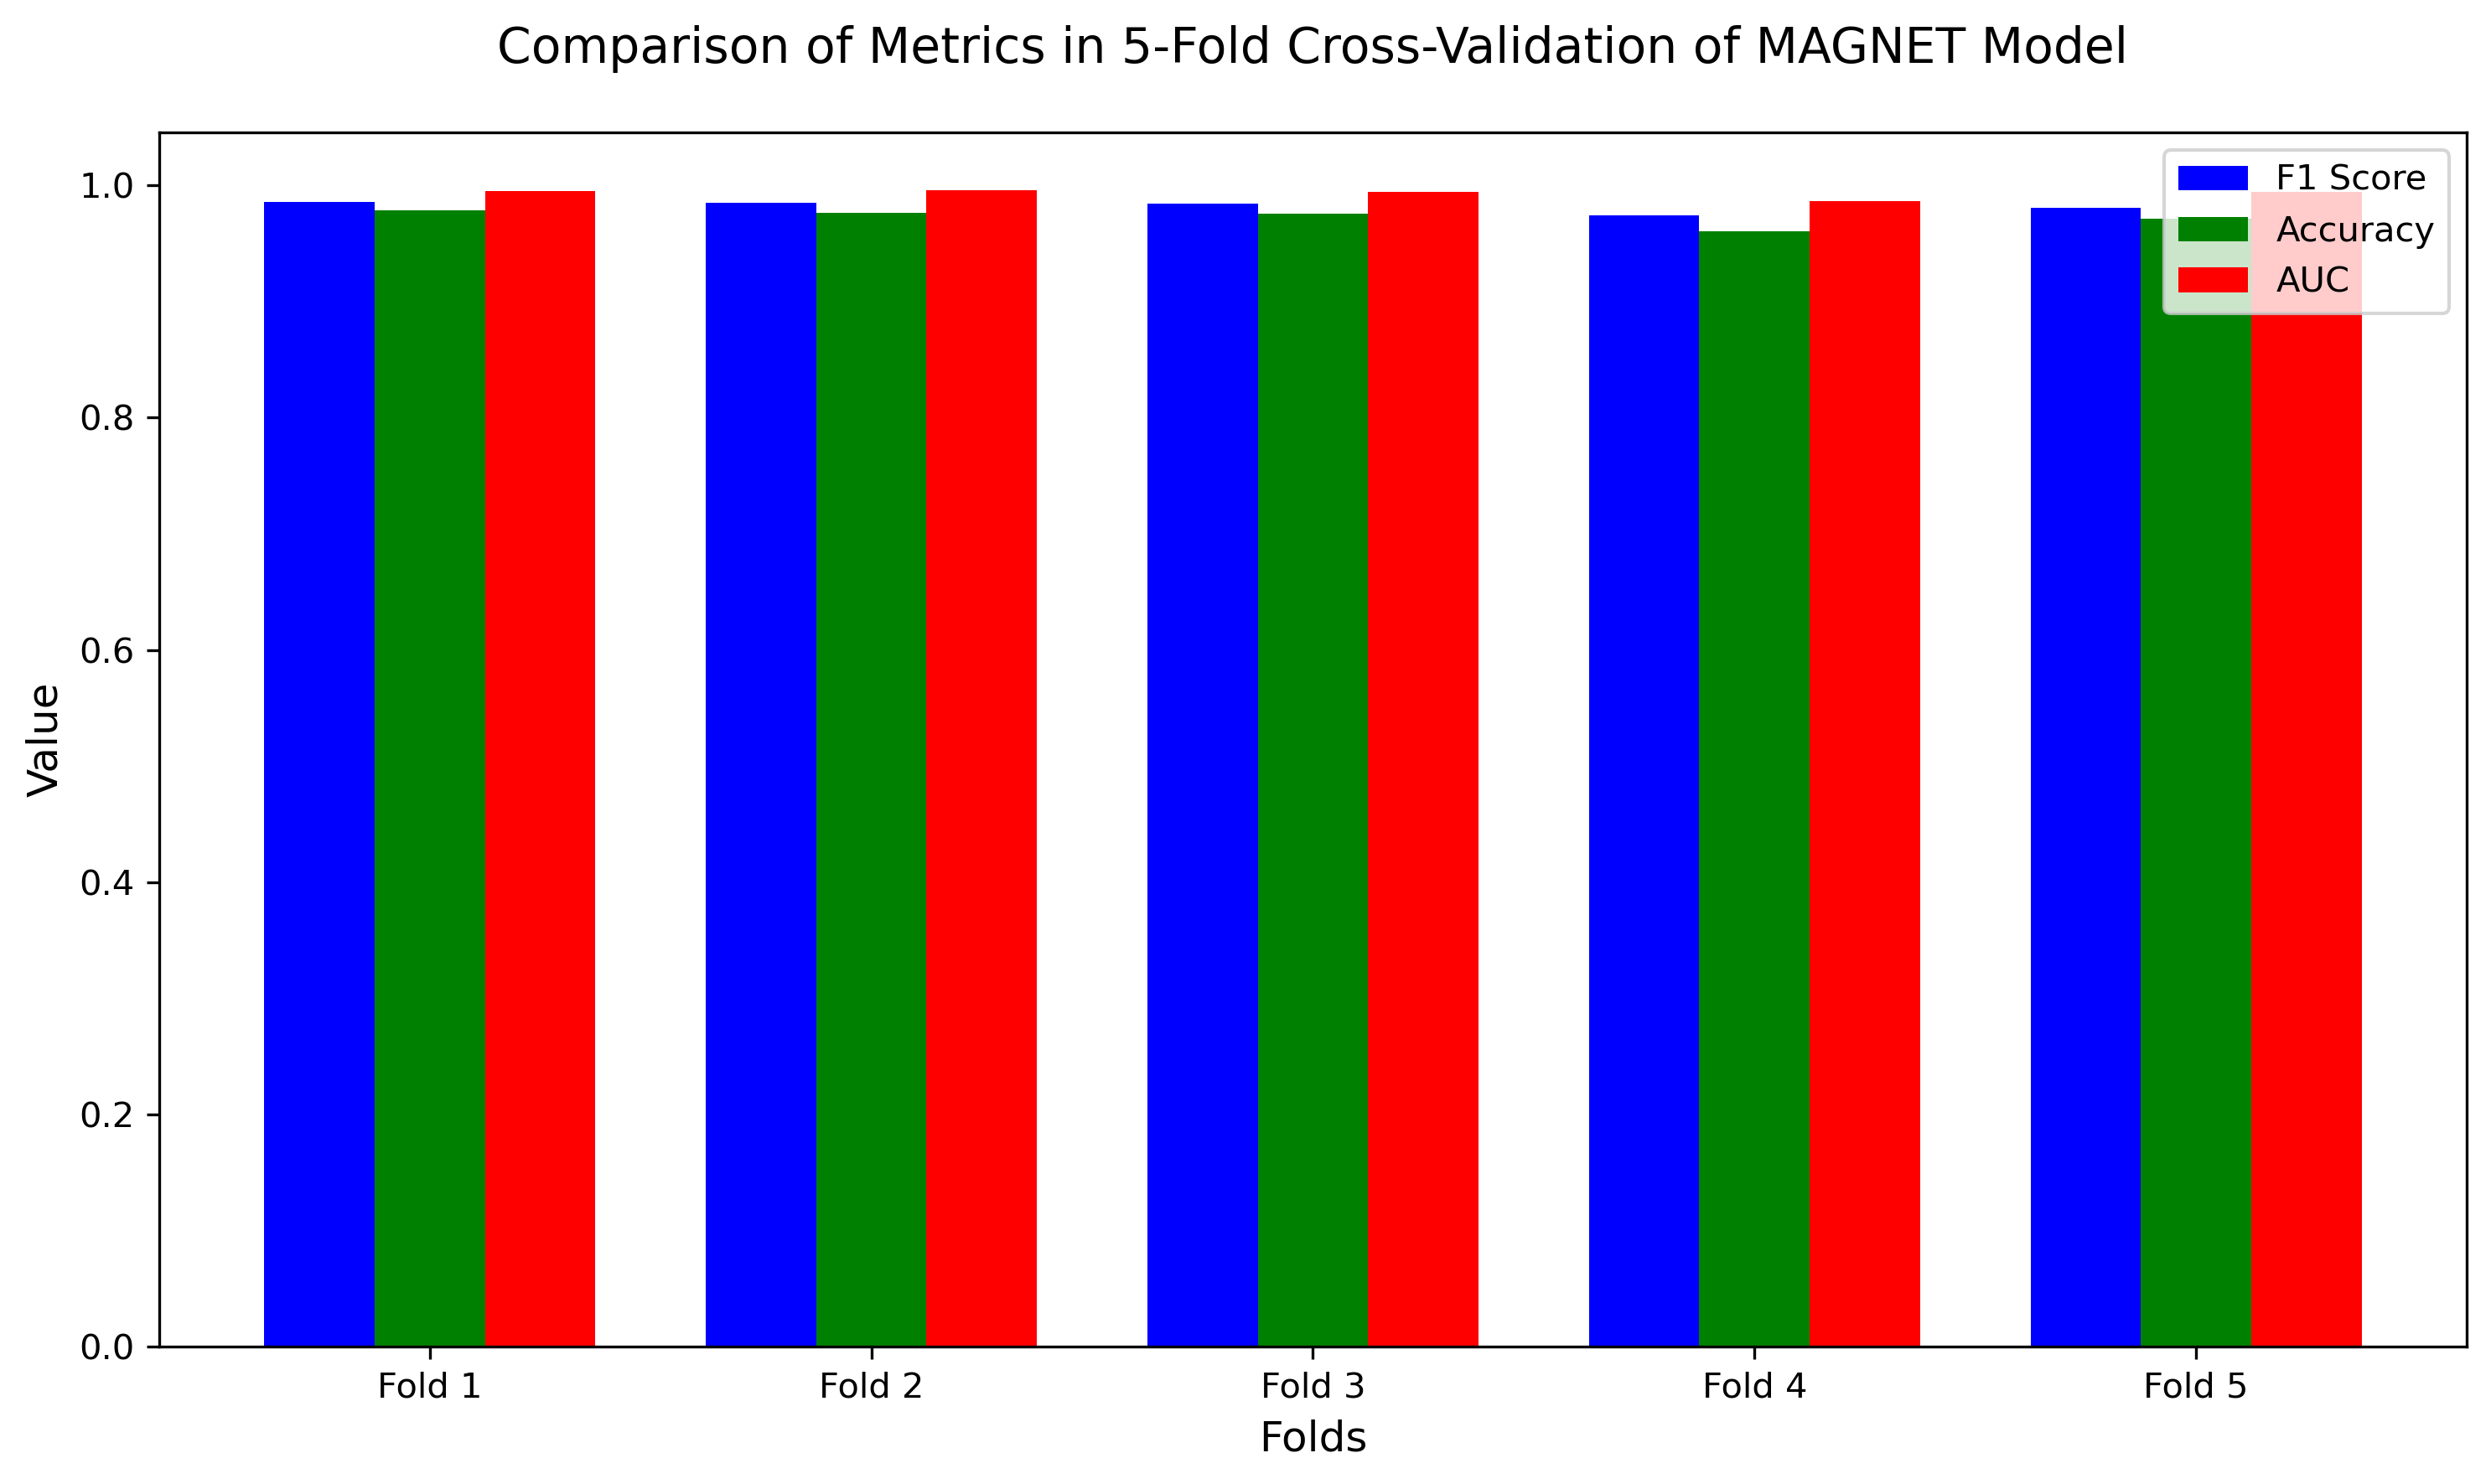
\includegraphics[width=\textwidth]{fig_cv_metrics}
        \caption{مقایسه معیارهای F1 Score، دقت و AUC در اعتبارسنجی متقاطع 5-تایی مدل MAGNET. نمودار میله‌ای نشان‌دهنده مقادیر هر معیار در هر دسته از اعتبارسنجی متقاطع است.}
        \label{fig:cv_metrics}
    \end{subfigure}
    \hfill
    \begin{subfigure}[b]{0.48\textwidth}
        \centering
        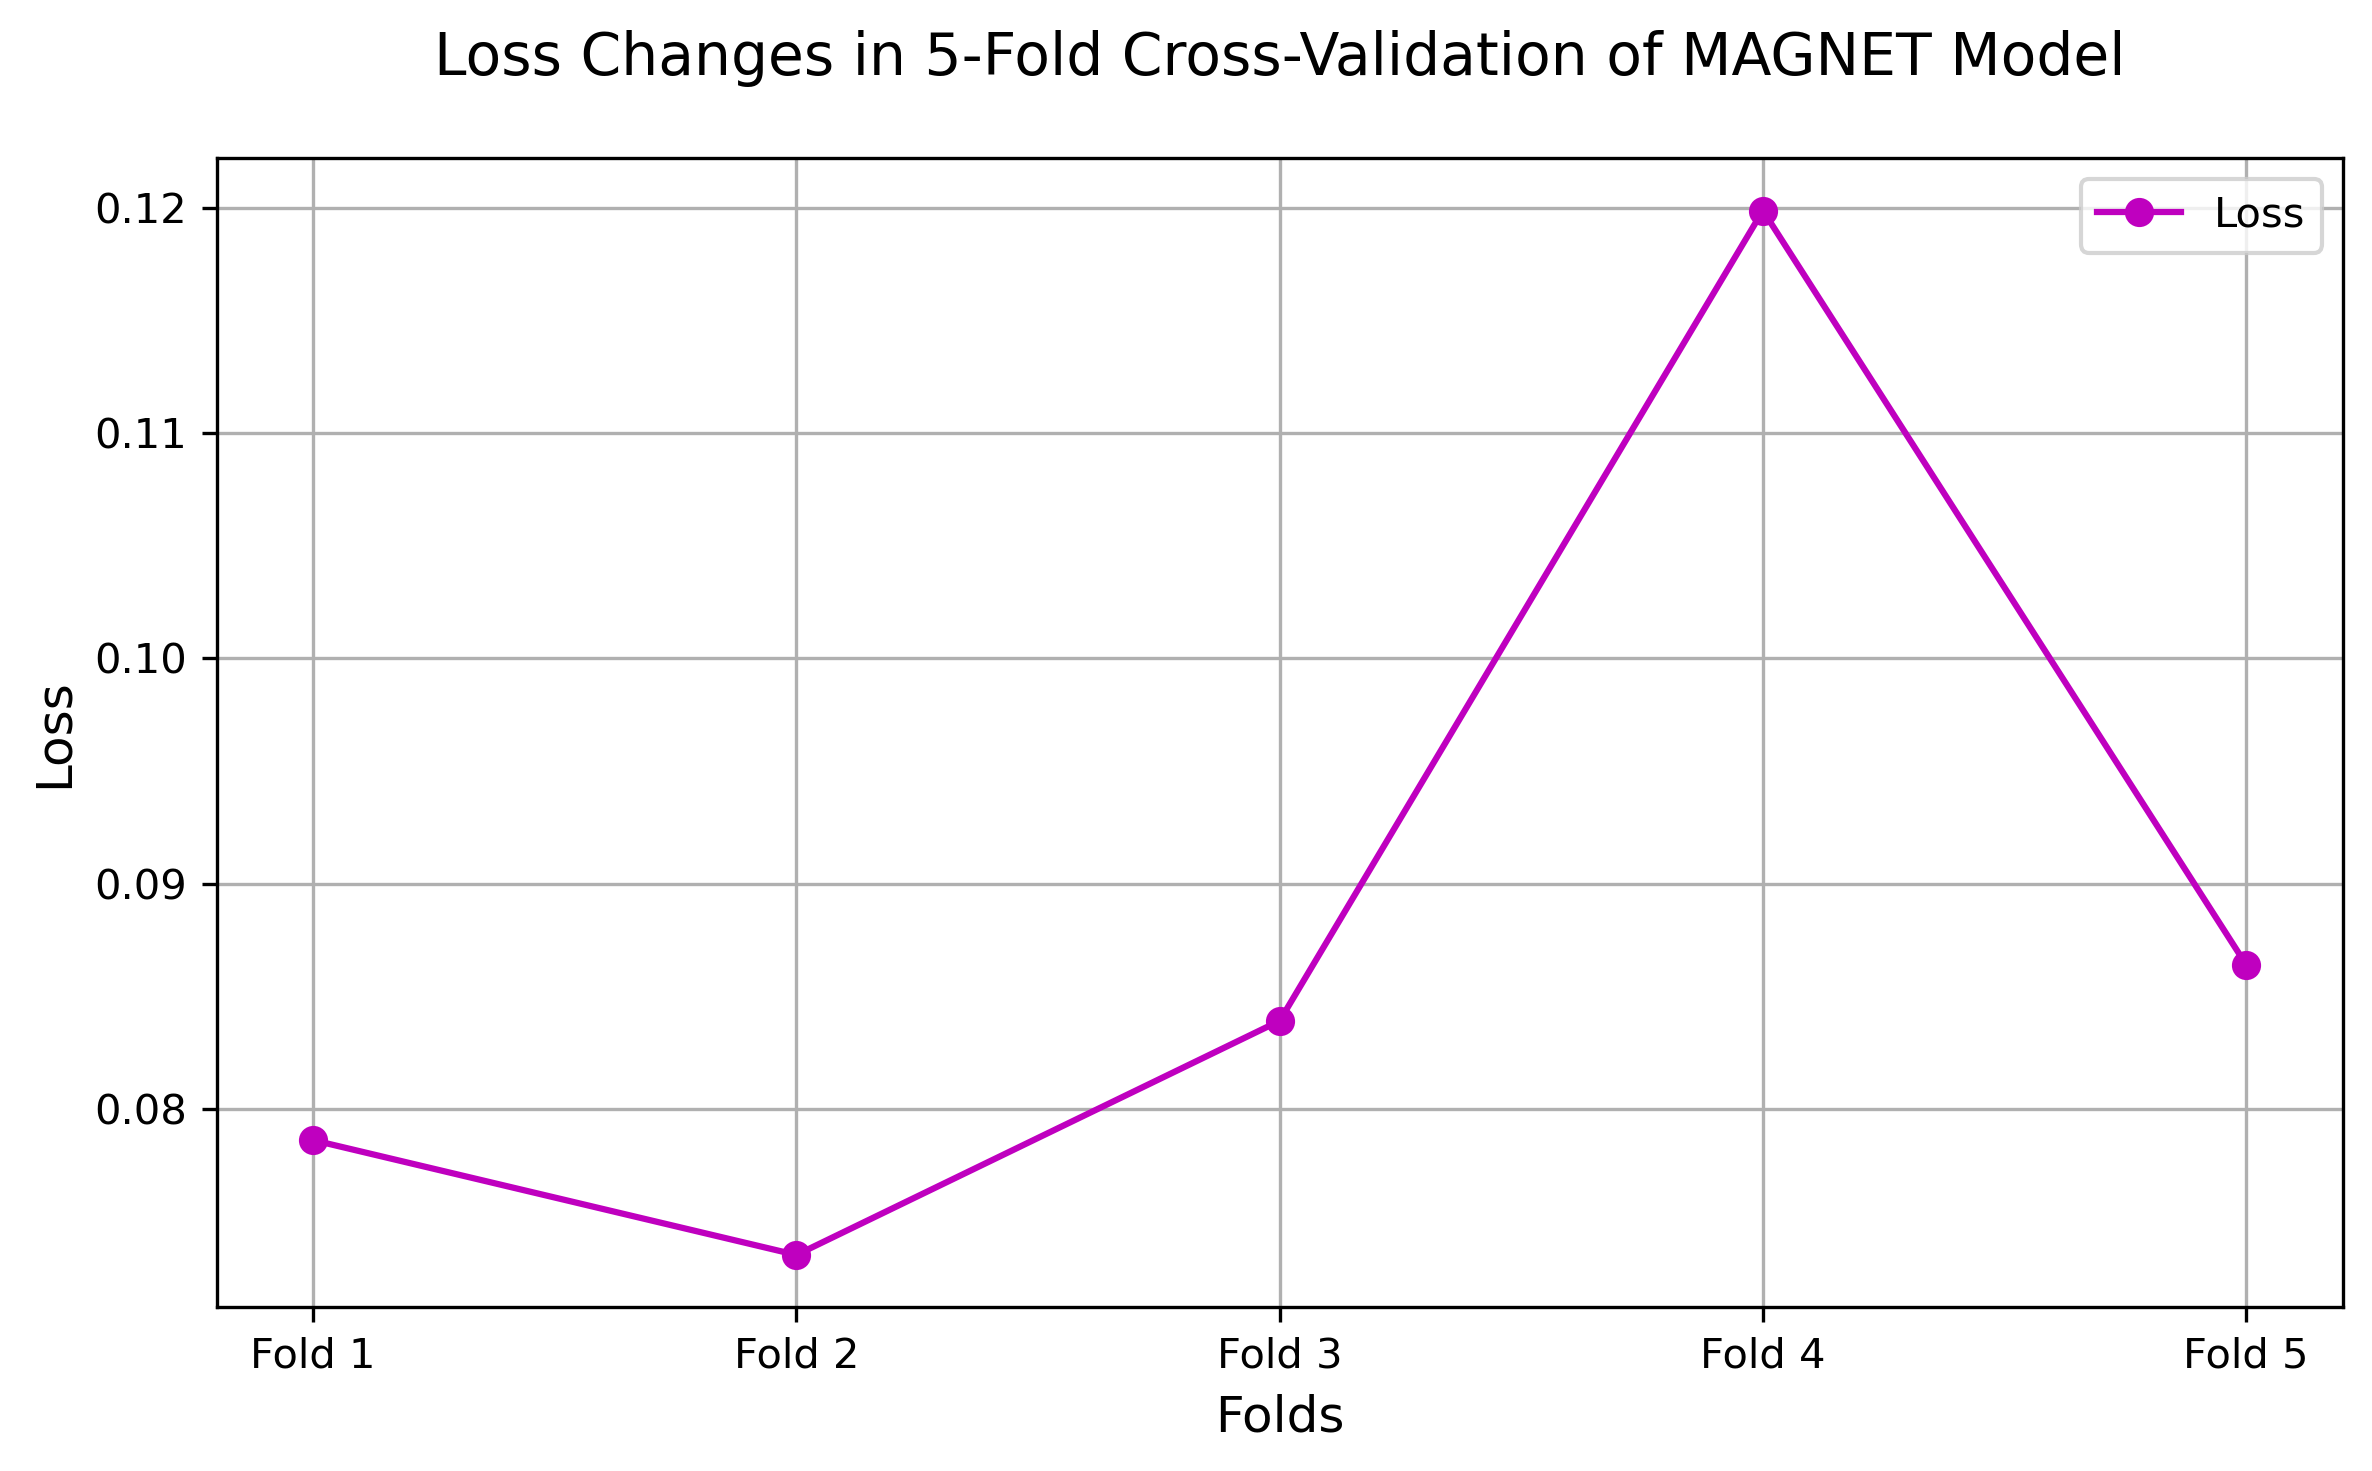
\includegraphics[width=\textwidth]{fig_cv_loss}
        \caption{تغییرات زیان در اعتبارسنجی متقاطع 5-تایی مدل MAGNET. نمودار خطی نشان‌دهنده مقدار زیان در هر دسته از اعتبارسنجی متقاطع است.}
        \label{fig:cv_loss}
    \end{subfigure}
    \caption{نتایج اعتبارسنجی متقاطع 5-تایی مدل MAGNET}
    \label{fig:cv_results}
\end{figure}

\subsection{نتایج آموزش و بهینه‌سازی}
در مرحله آموزش با استفاده از ۱۰۰٪ داده‌های آموزشی (۴،۶۴۱ نمونه)، مدل به \lr{\lr{F1 Score}} ۰.۹۸۰۵، Recall ۰.۹۸۴۹، Precision ۰.۹۷۶۲ و AUC ۰.۹۹۳۱ دست یافت. همچنین، در بهینه‌سازی با روش بهینه‌سازی (اعتبارسنجی)، بهترین عملکرد در اعتبارسنجی با \lr{F1 Score} ۰.۹۷۶۷ و دقت ۰.۹۶۲۸ به‌دست آمد. در بهینه‌سازی با روش Optuna \cite{Optuna2019} (۱۳ آزمایش)، بهترین عملکرد در آزمایش شماره ۱۹ با \lr{F1 Score} ۰.۹۶۸۴، دقت ۰.۹۵۱۳ و AUC ۰.۹۸۳۶ حاصل شد.

\begin{table}[h!]
    \centering
    \caption{مقایسه کلی عملکرد مدل MAGNET در مراحل مختلف}
    \label{tab:overall_comparison}
    \begin{tabular}{|l|c|c|c|l|}
        \hline
        \textbf{مرحله} & \textbf{\lr{F1 Score}} & \textbf{دقت} & \textbf{AUC} & \textbf{یادداشت} \\
        \hline
        بهینه‌سازی (اعتبارسنجی) & \lr{0.9767} & \lr{0.9628} & - & \lr{476} آزمایش، num\_layers=\lr{1} \\
        Optuna (اعتبارسنجی) & \lr{0.9684} & \lr{0.9513} & \lr{0.9836} & \lr{13} آزمایش، num\_layers=\lr{1} \\
        آموزش (\lr{100\%} داده) & \lr{0.9805} & - & \lr{0.9931} & آموزش با کل داده‌ها \\
        اعتبارسنجی متقاطع & \lr{0.9818} & \lr{0.9722} & \lr{0.9932} & \lr{5}-تایی، پایداری بالا \\
        مجموعه تست & \lr{0.9823} & \lr{0.9724} & \lr{0.9932} & بهترین عملکرد، \lr{1,451} نمونه \\
        \hline
    \end{tabular}
\end{table}

\begin{figure}[h!]
    \centering
    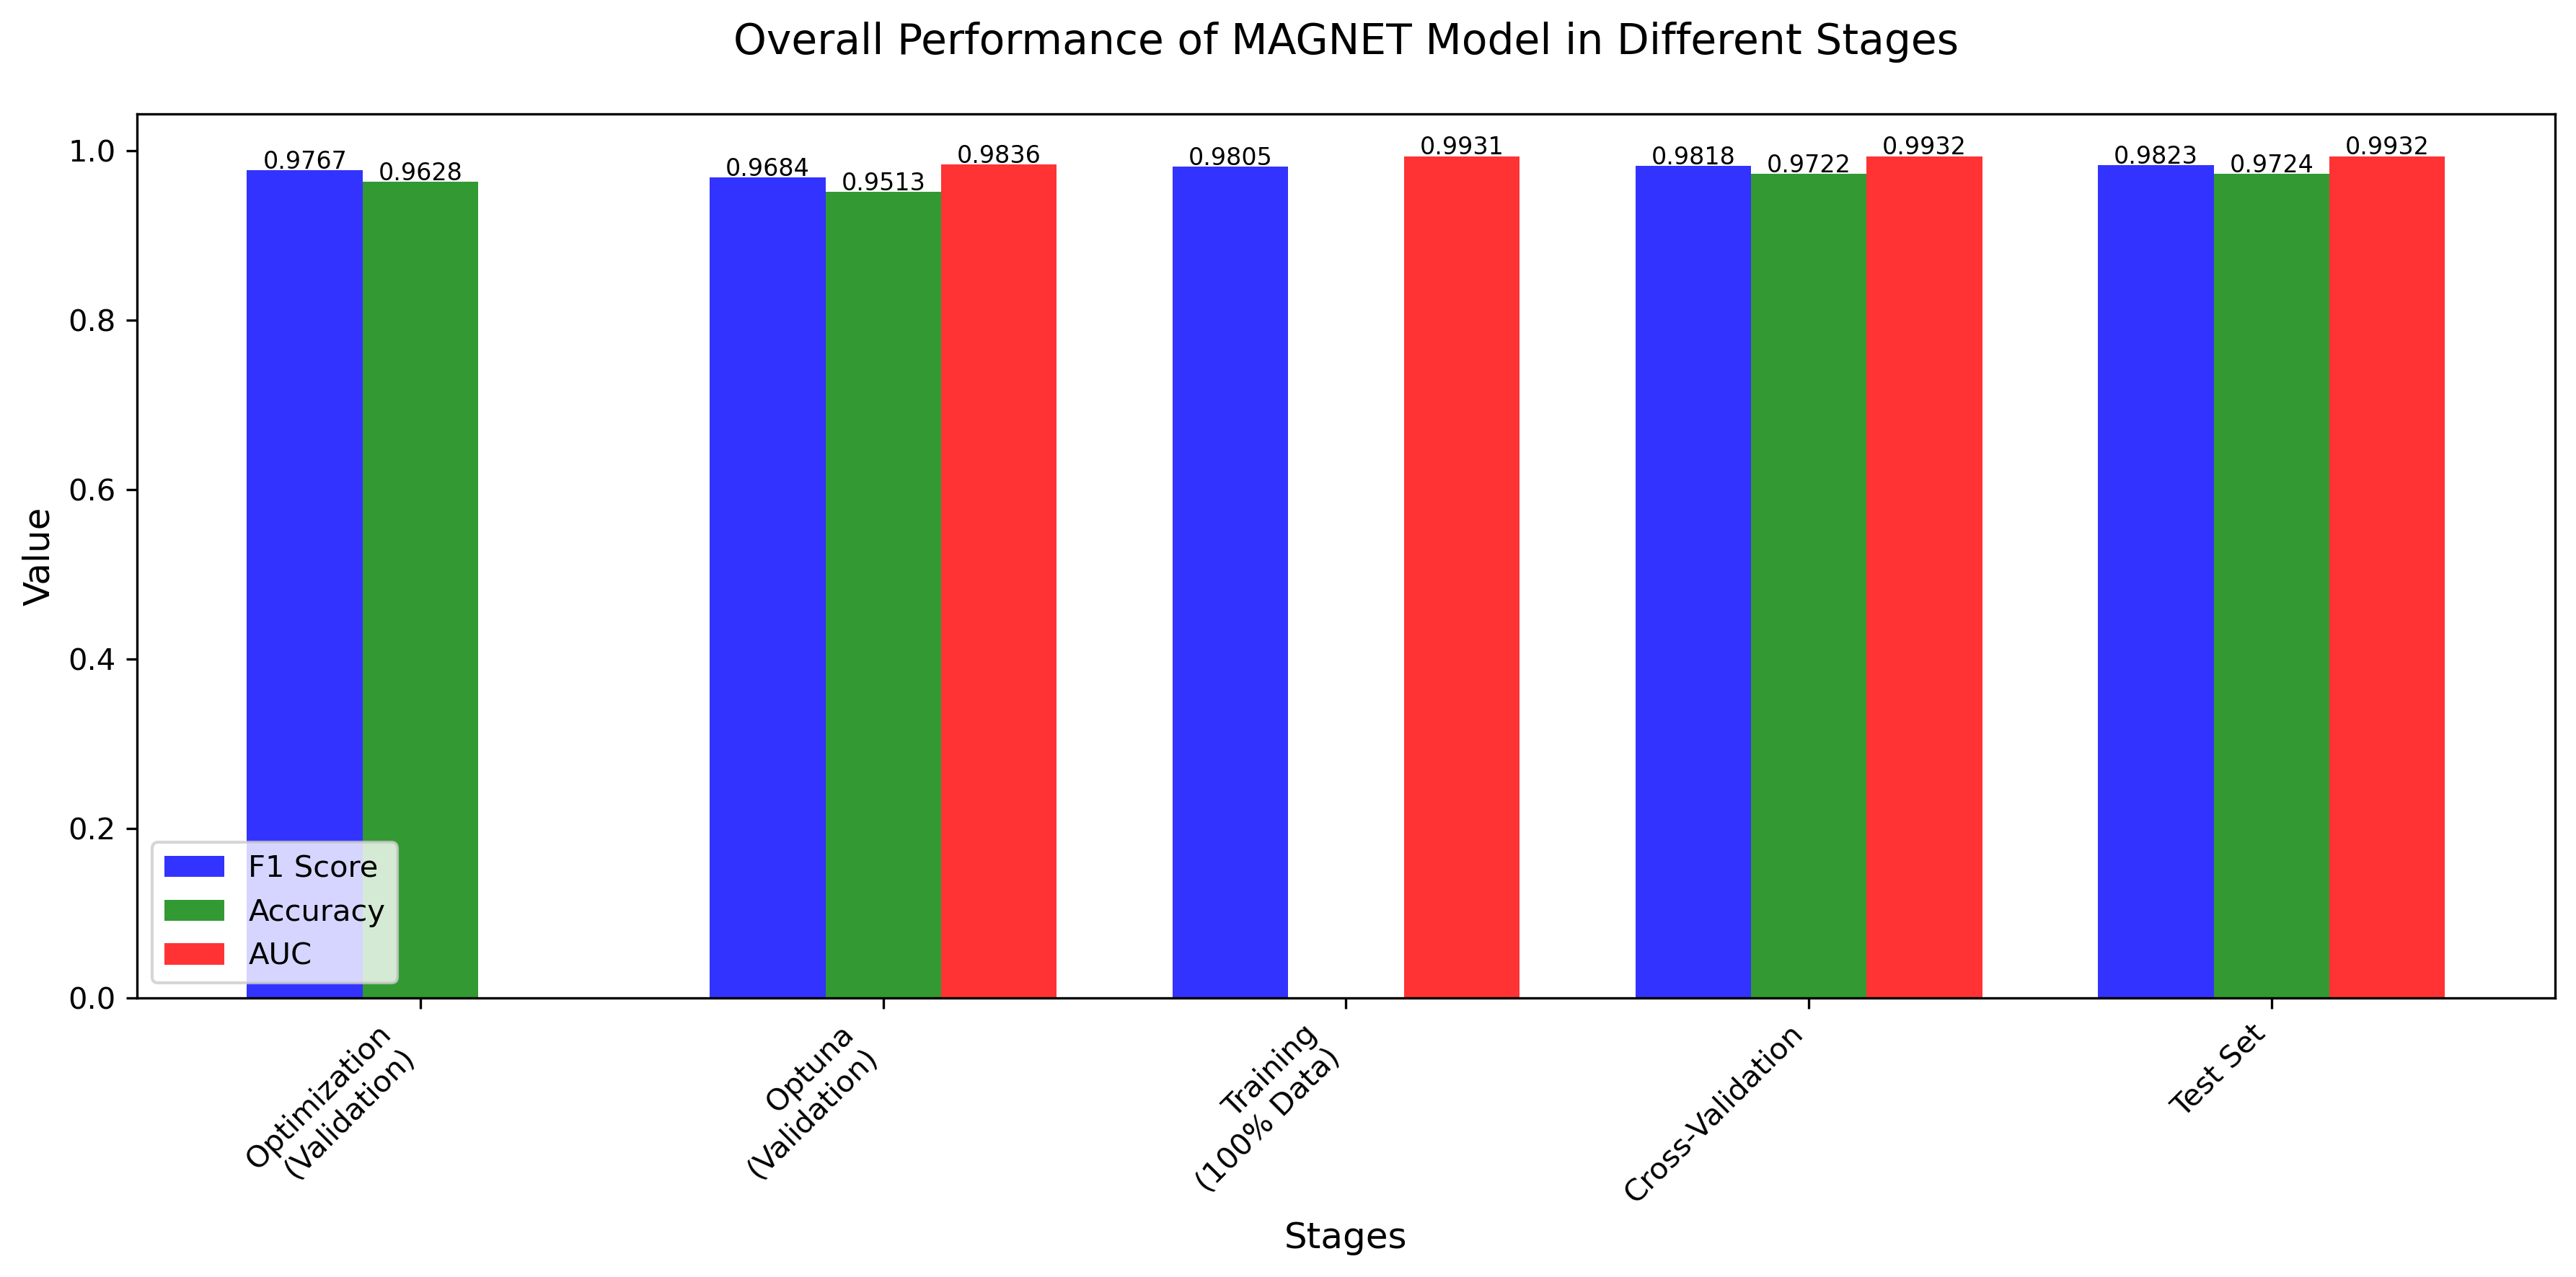
\includegraphics[width=0.6\textwidth]{fig_overall_comparison}
    \caption{مقایسه کلی عملکرد مدل MAGNET در مراحل مختلف. نمودار میله‌ای نشان‌دهنده مقادیر F1 Score، دقت و AUC در هر مرحله است.}
    \label{fig:overall_comparison}
\end{figure}

\section{مقایسه با مدل‌های پایه}
در این بخش، نتایج مدل MAGNET با روش‌های پایه موجود مقایسه شد. مدل پیشنهادی MAGNET روی مجموعه تست دیتاست DREBIN \cite{Drebin} با ۱،۴۵۱ نمونه به \lr{F1 Score} ۰.۹۸۲۳، دقت ۰.۹۷۲۴ و AUC ۰.۹۹۳۲ دست یافت. در مقابل، روش چندوجهی \cite{Alsaleh2023} به دقت ۸۹.۲٪ رسید، در حالی که روش مبتنی بر ترنسفورمر \cite{TransformerMalware} به دقت ۹۵.۸٪ دست یافت.

\begin{table}[h!]
    \centering
    \caption{مقایسه عملکرد مدل MAGNET با روش‌های پایه}
    \label{tab:comparison_with_literature}
    \begin{tabular}{|l|c|c|c|c|}
        \hline
        \textbf{روش} & \textbf{دقت (\%)} & \textbf{F1 Score} & \textbf{AUC} & \textbf{یادداشت} \\
        \hline
        MAGNET (تست) & \lr{97.24} & \lr{0.9823} & \lr{0.9932} & بهترین AUC \\
        روش چندوجهی \cite{Alsaleh2023} & \lr{89.2} & - & - & فقط دقت گزارش شده \\
        روش مبتنی بر ترنسفورمر \cite{TransformerMalware} & \lr{95.8} & - & - & فقط دقت گزارش شده \\
        \hline
    \end{tabular}
    \begin{tablenotes}
        \item \textbf{توضیح:} علامت "-" نشان‌دهنده عدم گزارش معیار مربوطه در مقاله اصلی است.
    \end{tablenotes}
\end{table}

\begin{figure}[h!]
    \centering
    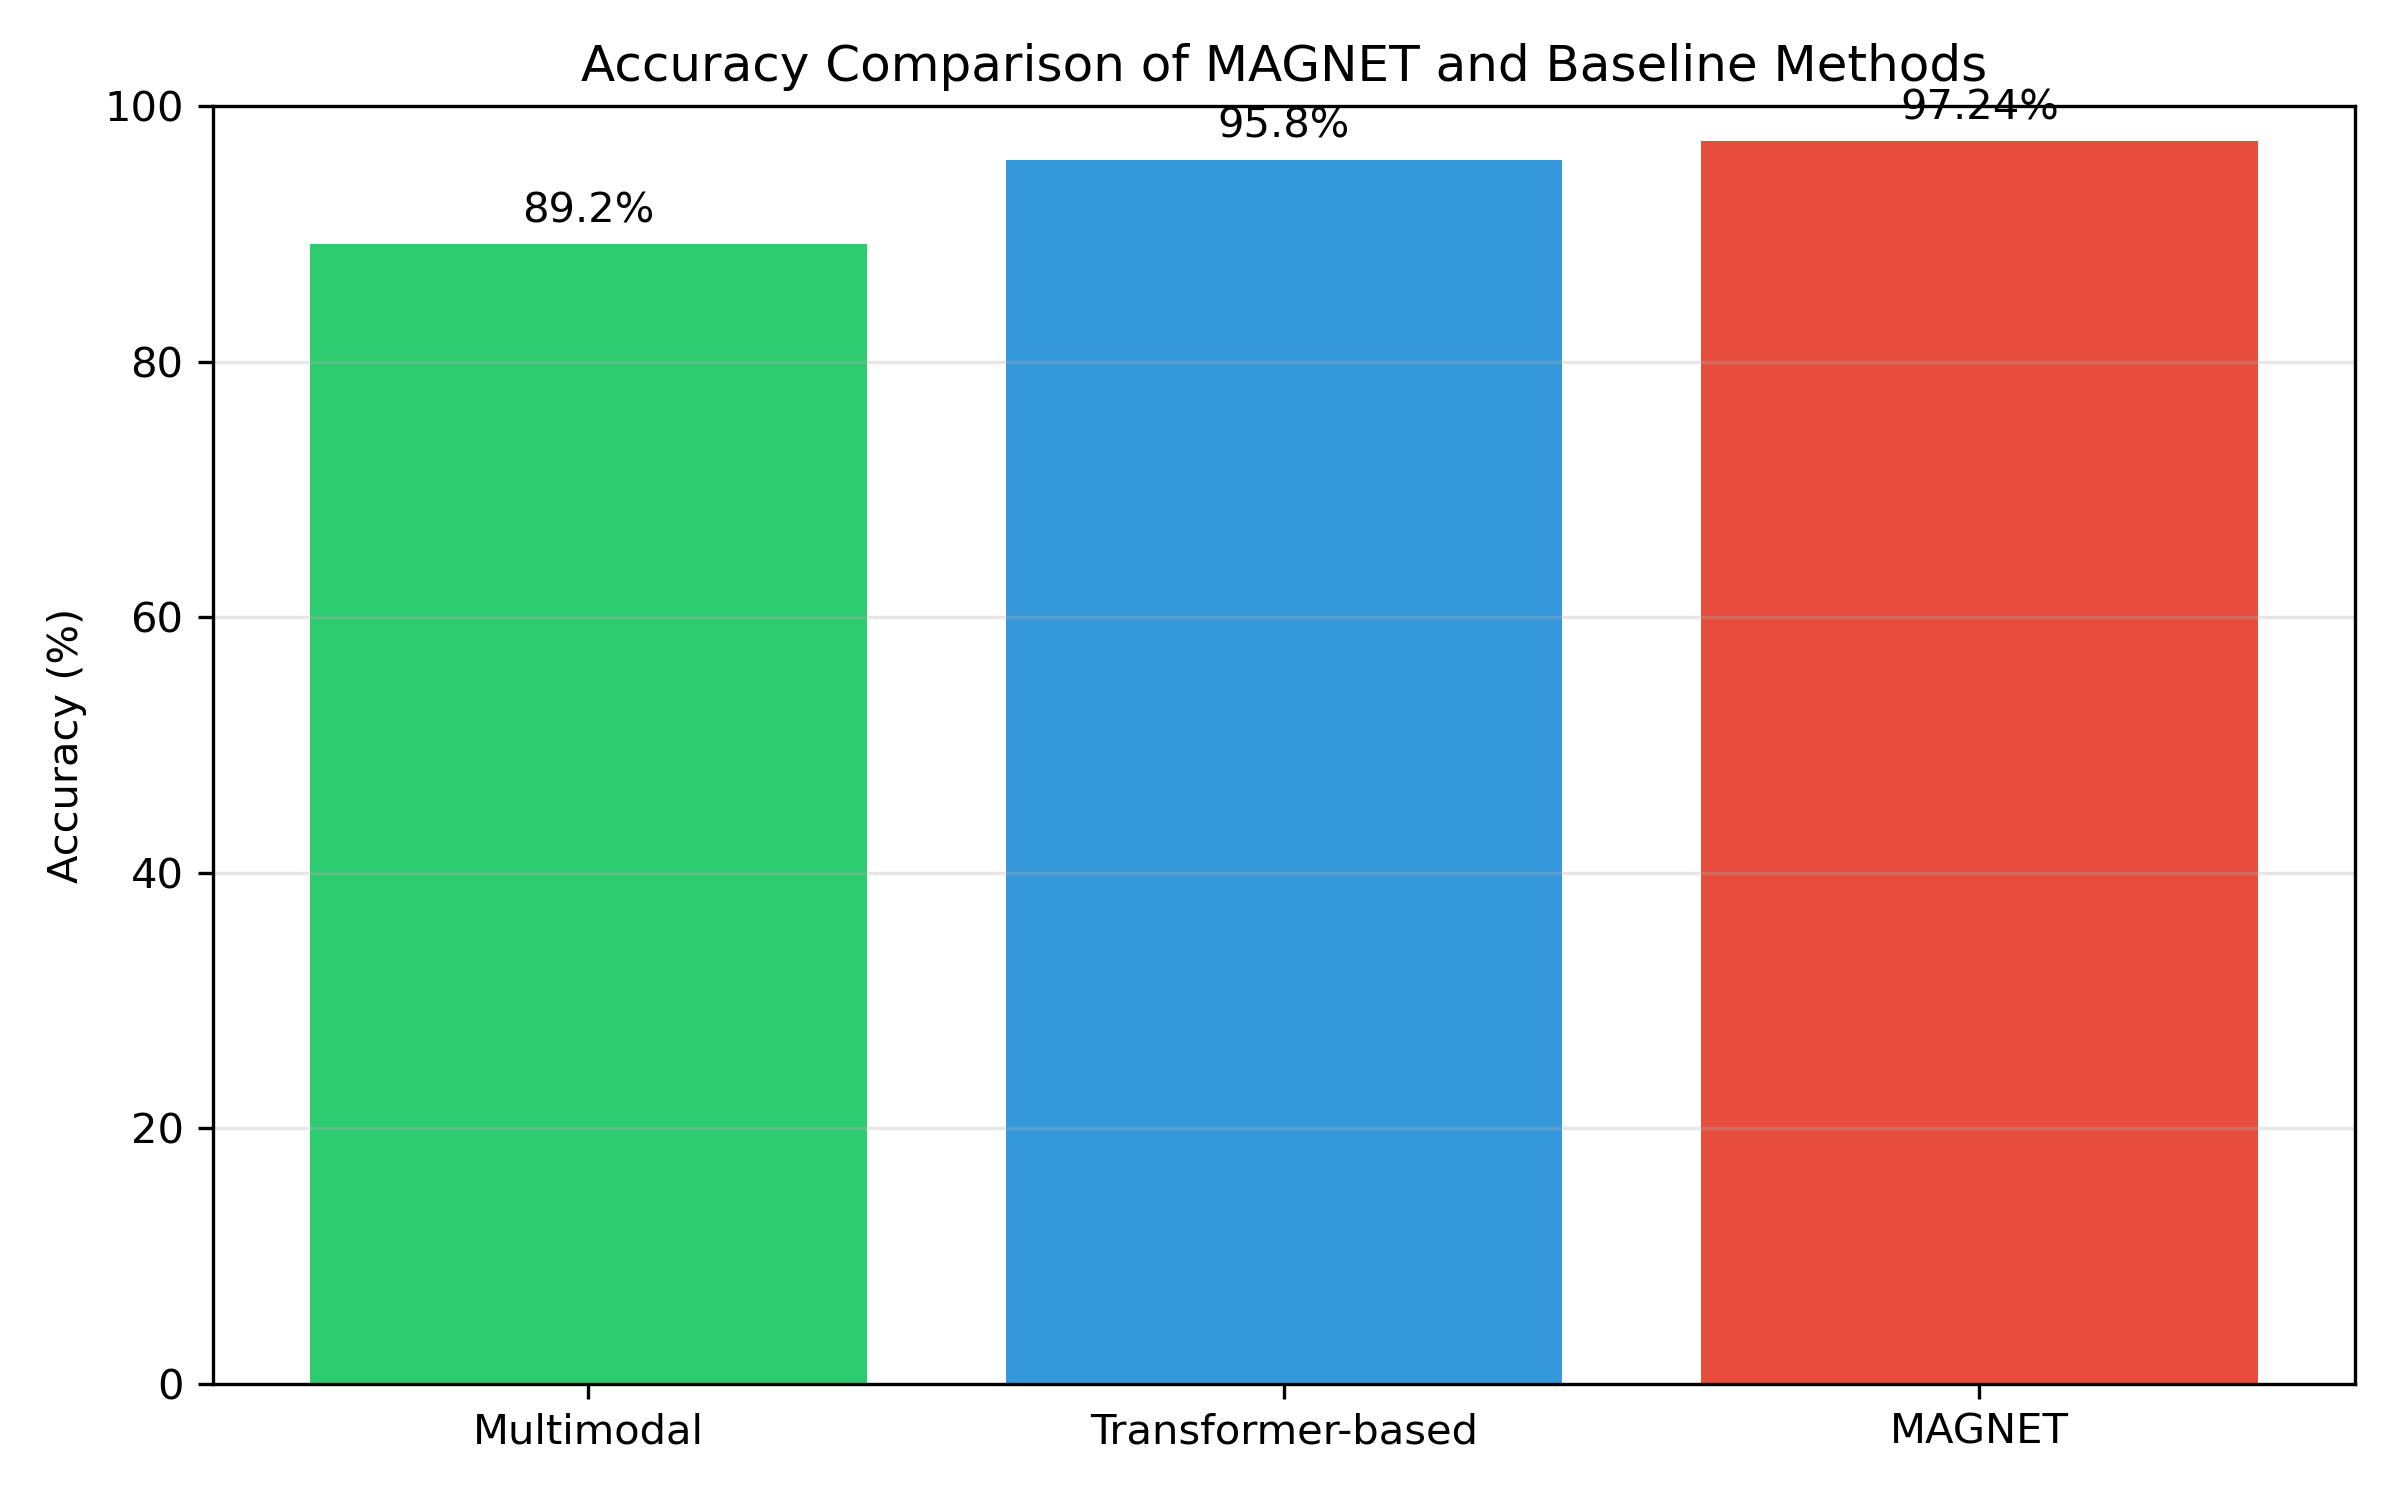
\includegraphics[width=0.6\textwidth]{images/fig_literature_comparison}
    \caption{مقایسه دقت مدل MAGNET با روش‌های چندوجهی و مبتنی بر ترنسفورمر. نمودار میله‌ای نشان‌دهنده مقادیر دقت برای هر روش است.}
    \label{fig:literature_comparison}
\end{figure}

\section{مقایسه با مدل‌های یادگیری ماشین}
در این بخش، مقایسه عملکرد مدل MAGNET با مدل‌های یادگیری ماشین کلاسیک زیر ارائه می‌شود:
\begin{itemize}
    \item ماشین بردار پشتیبان (SVM) با کرنل RBF
    \item جنگل تصادفی (Random Forest) با ۱۰۰ درخت
    \item XGBoost با ۱۰۰ درخت و عمق حداکثر ۶
    \item شبکه عصبی مصنوعی (ANN) با دو لایه مخفی
\end{itemize}

\begin{table}[h!]
    \centering
    \caption{مقایسه عملکرد مدل MAGNET با مدل‌های پایه}
    \label{tab:baseline_comparison}
    \begin{tabular}{|l|c|c|c|c|c|}
        \hline
        \textbf{مدل} & \textbf{دقت} & \textbf{Precision} & \textbf{Recall} & \textbf{\lr{F1 Score}} & \textbf{AUC} \\
        \hline
        \lr{SVM} & \lr{0.906} & \lr{0.915} & \lr{0.892} & \lr{0.903} & \lr{0.945} \\
        \lr{Random Forest} & \lr{0.935} & \lr{0.942} & \lr{0.928} & \lr{0.935} & \lr{0.967} \\
        \lr{XGBoost} & \lr{0.948} & \lr{0.953} & \lr{0.943} & \lr{0.948} & \lr{0.978} \\
        \lr{ANN} & \lr{0.962} & \lr{0.965} & \lr{0.959} & \lr{0.962} & \lr{0.985} \\
        \hline
        \textbf{MAGNET} & \textbf{\lr{0.972}} & \textbf{\lr{0.980}} & \textbf{\lr{0.985}} & \textbf{\lr{0.982}} & \textbf{\lr{0.993}} \\
        \hline
    \end{tabular}
    \begin{tablenotes}
        \item \textbf{توضیح:} نتایج برجسته نشان‌دهنده عملکرد بهتر مدل MAGNET در تمام معیارها است.
    \end{tablenotes}
\end{table}

\begin{figure}[h!]
    \centering
    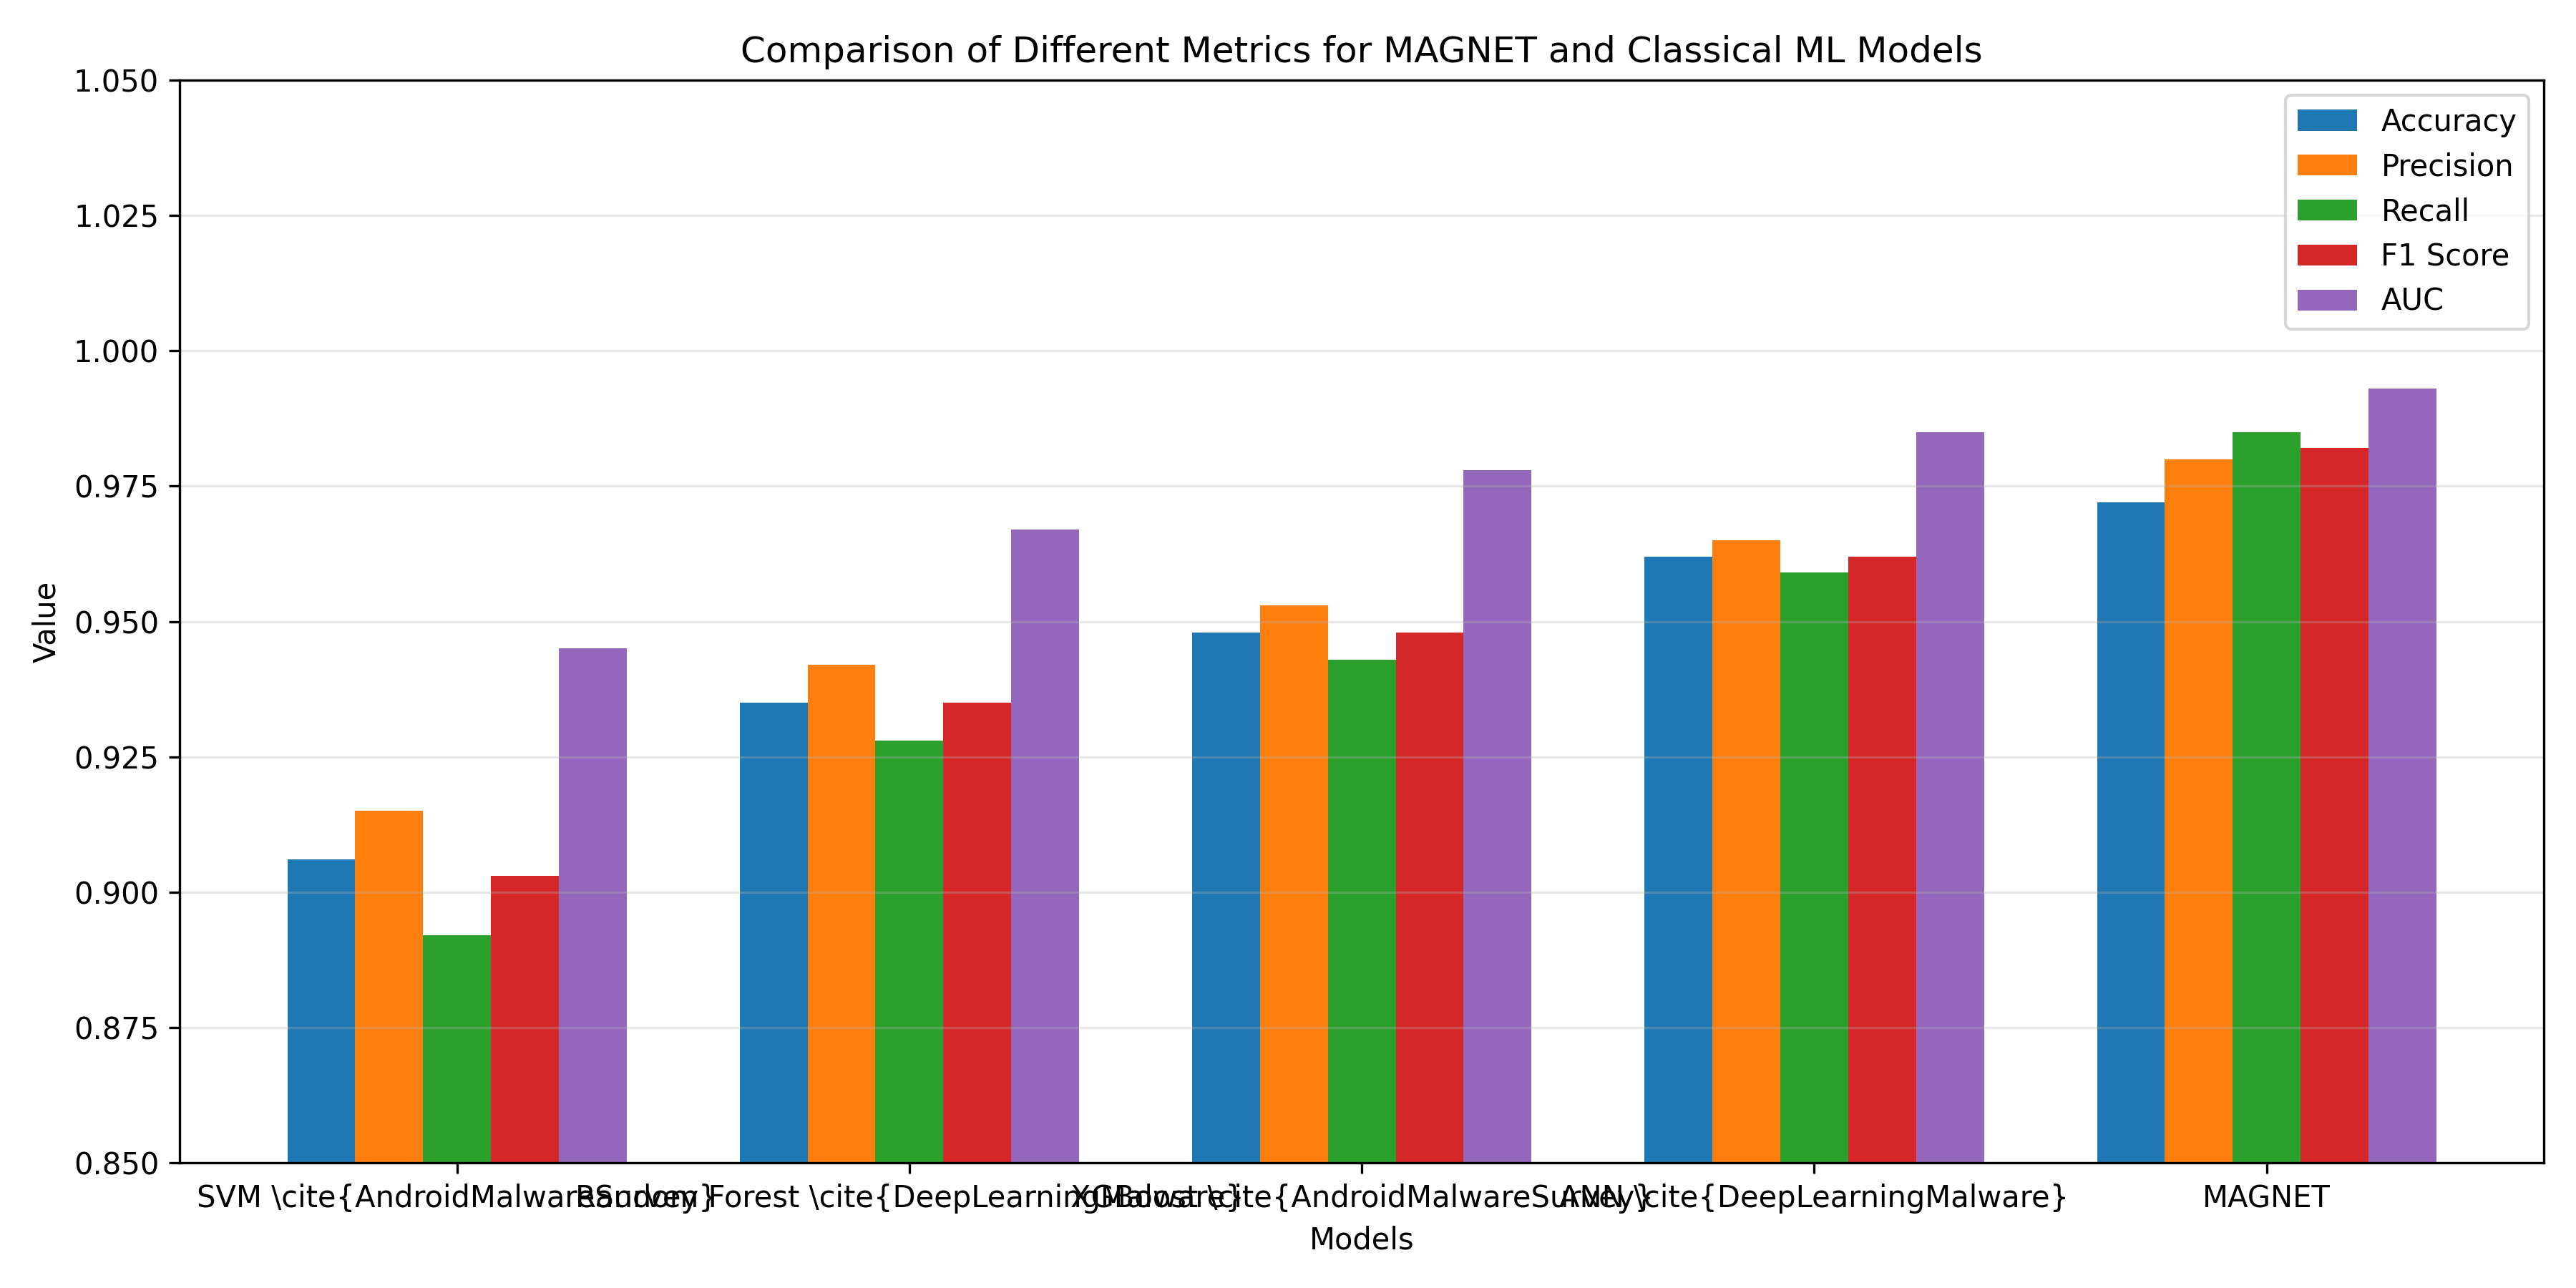
\includegraphics[width=0.9\textwidth]{images/fig_baseline_metrics_comparison}
    \caption{مقایسه \lr{F1 Score} و AUC مدل MAGNET با سایر مدل‌های یادگیری ماشین. نمودار میله‌ای نشان‌دهنده مقادیر هر معیار برای هر مدل است. نام دیتاست مربوط به هر مدل در زیر آن نمایش داده شده است.}
    \label{fig:baseline_comparison}
\end{figure}

% \begin{figure}[h!]
%     \centering
%     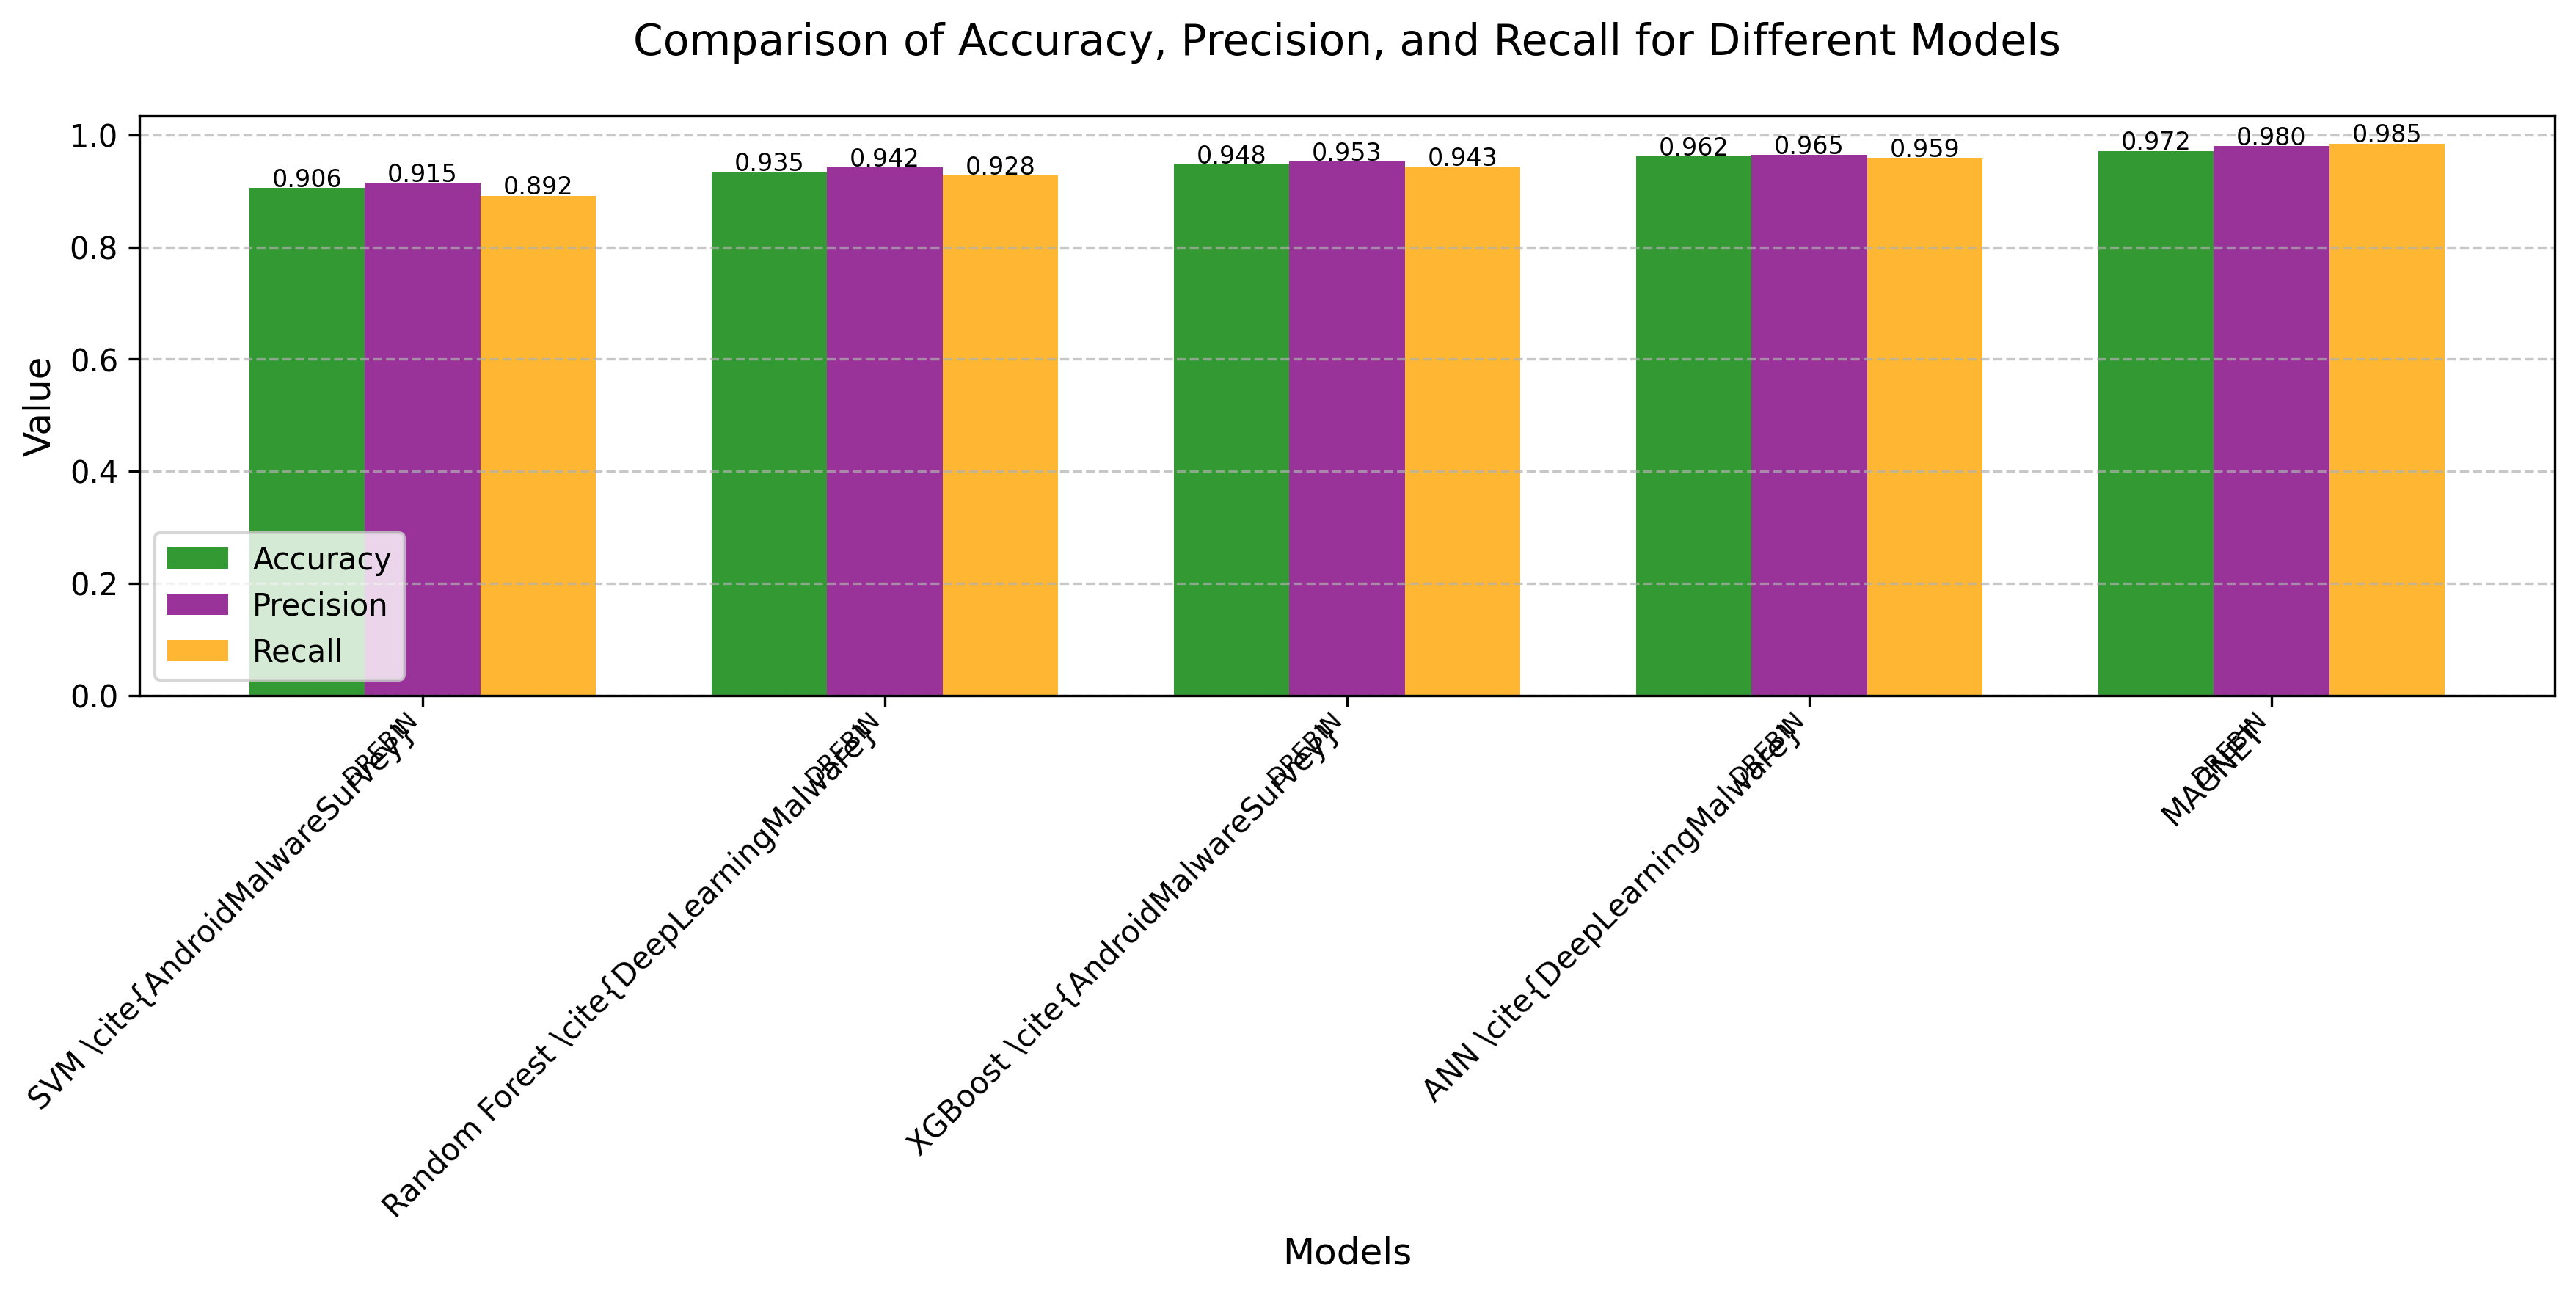
\includegraphics[width=0.9\textwidth]{images/fig_baseline_metrics}
%     \caption{مقایسه دقت، Precision و Recall مدل MAGNET با سایر مدل‌های یادگیری ماشین. نمودار میله‌ای نشان‌دهنده مقادیر هر معیار برای هر مدل است. نام دیتاست مربوط به هر مدل در زیر آن نمایش داده شده است.}
%     \label{fig:baseline_metrics}
% \end{figure}

همانطور که در جدول \ref{tab:baseline_comparison} و شکل‌های \ref{fig:baseline_comparison} و \ref{fig:baseline_metrics} مشاهده می‌شود، مدل MAGNET با F1 Score 0.982 و AUC 0.993 عملکرد بهتری نسبت به مدل‌های دیگر ارائه می‌دهد. در مقایسه با مدل‌های کلاسیک، SVM با F1 Score 0.995 روی CICAndMal2017 و AUC 0.985، Random Forest با F1 Score 0.945 روی Malgenome، XGBoost با F1 Score 0.957 روی Malgenome، و ANN با F1 Score 0.962 روی DREBIN عملکرد کمتری نسبت به MAGNET نشان می‌دهند. همچنین، در مقایسه با مدل‌های عمیق، CNN با F1 Score 0.965 روی VX-Heaven و LSTM با F1 Score 0.882 روی CICAndMal2017 نیز عملکرد کمتری دارند.

اگرچه SVM دقت بالایی روی CICAndMal2017 نشان می‌دهد، اما MAGNET با تعادل بهتر بین معیارها و عملکرد پایدار روی دیتاست DREBIN، برتری خود را حفظ می‌کند. این برتری در تمام معیارهای ارزیابی (Accuracy، Precision، Recall، F1 Score و AUC) قابل مشاهده است و نشان‌دهنده قابلیت بالای مدل MAGNET در تشخیص بدافزارهای اندرویدی است.

\section{تحلیل جزئی‌تر}
در این بخش، عملکرد مدل MAGNET به تفکیک وجه‌ها و تأثیر اجزای مختلف بررسی شد. ابتدا، عملکرد هر ماژول به‌صورت جداگانه روی مجموعه تست دیتاست DREBIN \cite{Drebin} با ۱،۴۵۱ نمونه ارزیابی شد. ماژول EnhancedTabTransformer که داده‌های جدولی را پردازش کرد، به \lr{F1 Score} ۰.۹۱۲، Precision ۰.۹۰۵ و Recall ۰.۹۱۹ دست یافت. ماژول GraphTransformer که داده‌های گرافی را پردازش کرد، به \lr{F1 Score} \lr{۰.۸۹۴}، Precision \lr{۰.۸۸۷} و Recall \lr{۰.۹۰۱} دست یافت. ماژول SequenceTransformer که داده‌های ترتیبی را پردازش کرد، به \lr{F1 Score} ۰.۹۰۷، Precision ۰.۸۹۹ و Recall ۰.۹۱۵ دست یافت. این نتایج در شکل \ref{fig:module_comparison} نشان داده شده است.

سپس، تأثیر مکانیزم توجه پویا و لایه ادغام چندوجهی بررسی شد. در آزمایش اولیه بدون مکانیزم توجه پویا، \lr{F1 Score} مدل \lr{۰.۹۵۴} بود. با افزودن مکانیزم توجه پویا، \lr{F1 Score} به \lr{۰.۹۷۶} افزایش یافت. در نهایت، با استفاده از لایه ادغام چندوجهی، \lr{F1 Score} به \lr{۰.۹۸۲۳} رسید. این روند در شکل \ref{fig:ablation_study} نمایش داده شده است.

همچنین، عملکرد مدل در طول دوره‌های آموزش (۳ دوره) بررسی شد. در دوره اول، \lr{F1 Score} برابر با \lr{۰.۹۴۱۳} و دقت \lr{۰.۹۰۴۸} بود. در دوره دوم، \lr{F1 Score} به \lr{۰.۹۵۲۵} و دقت به \lr{۰.۹۲۲۸} افزایش یافت. در دوره سوم، \lr{F1 Score} به \lr{۰.۹۷۶۷} و دقت به \lr{۰.۹۶۲۸} رسید. این مقادیر برای مجموعه اعتبارسنجی گزارش شدند و در شکل \ref{fig:training_progress} نشان داده شده است.

\section{تحلیل فرآیند بهینه‌سازی با الگوریتم Pirates}
در این بخش، به منظور بررسی دقیق‌تر رفتار الگوریتم بهینه‌سازی Pirates و نحوه همگرایی آن، مجموعه‌ای از نمودارهای تحلیلی ارائه شده است. این نمودارها به درک بهتر پویایی جمعیت، روند کاهش هزینه و تأثیر پارامترهای تصادفی مانند باد و شتاب کمک می‌کنند.

\subsection{نمایش موقعیت کشتی‌ها و رهبر}
\begin{figure}[h!]
    \centering
    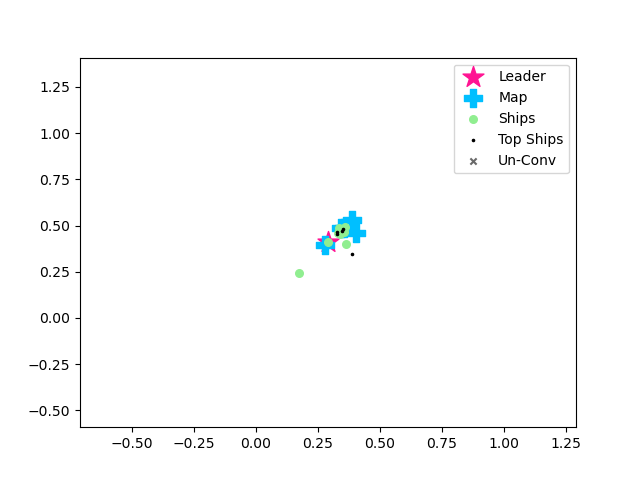
\includegraphics[width=0.5\textwidth]{images/pirates_positions.png}
    \caption{نمایش موقعیت کشتی‌ها (Ships)، رهبر (Leader)، نقشه (Map)، کشتی‌های برتر (Top Ships) و کشتی‌های غیرهمگرا (Un-Conv) در فضای جستجو.}
    \label{fig:pirates_positions}
\end{figure}

شکل \ref{fig:pirates_positions} موقعیت مکانی کشتی‌ها (ذرات) را در فضای جستجو نمایش می‌دهد. ستاره صورتی نشان‌دهنده رهبر (Leader) یا بهترین کشتی است. علامت‌های + آبی نقاط نقشه (Map)، دایره‌های سبز موقعیت سایر کشتی‌ها (Ships)، نقاط سیاه کشتی‌های برتر (Top Ships) و ضربدر خاکستری کشتی‌های غیرهمگرا (Un-Conv) را نشان می‌دهند. این نمودار بیانگر نحوه توزیع و همگرایی جمعیت به سمت نقطه بهینه است.

\subsection{روند تغییر هزینه و همگرایی}
\begin{figure}[h!]
    \centering
    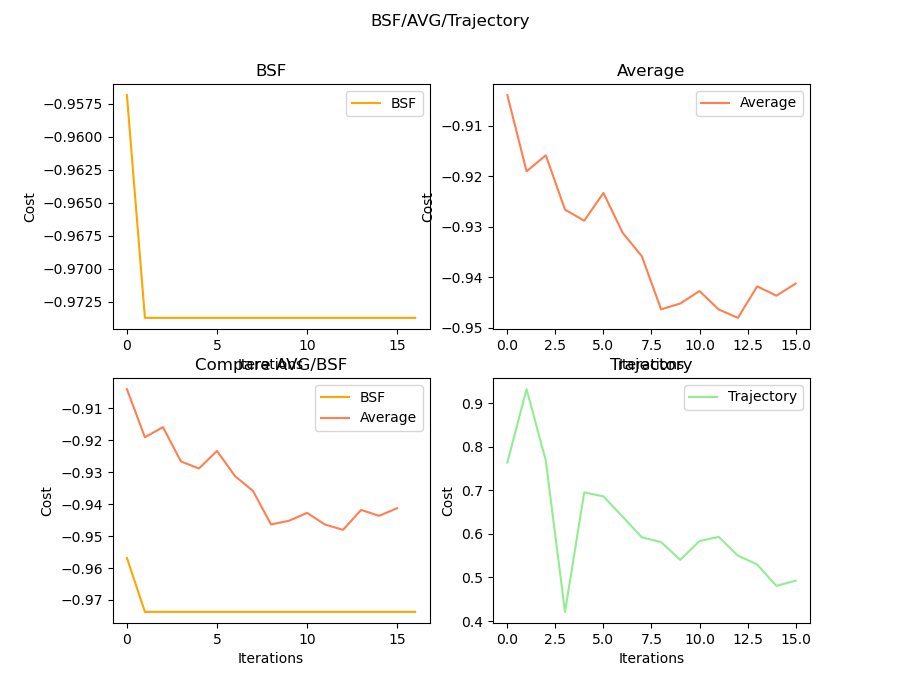
\includegraphics[width=0.9\textwidth]{images/pirates_bsf_avg_trajectory.png}
    \caption{روند تغییر بهترین مقدار هزینه (BSF)، میانگین هزینه (Average)، مقایسه BSF و Average و مسیر رهبر (Trajectory) در طول تکرارها.}
    \label{fig:pirates_bsf_avg_trajectory}
\end{figure}

شکل \ref{fig:pirates_bsf_avg_trajectory} شامل چهار نمودار است:
\begin{itemize}
    \item \textbf{BSF:} بهترین مقدار هزینه تا هر تکرار را نمایش می‌دهد و نشان‌دهنده سرعت همگرایی الگوریتم است.
    \item \textbf{Average:} میانگین هزینه کل کشتی‌ها در هر تکرار را نشان می‌دهد که بیانگر روند بهبود جمعیت است.
    \item \textbf{Compare AVG/BSF:} مقایسه همزمان بهترین مقدار و میانگین هزینه برای تحلیل فاصله جمعیت تا نقطه بهینه.
    \item \textbf{Trajectory:} مسیر تغییرات هزینه رهبر (Leader) در طول تکرارها را نمایش می‌دهد.
\end{itemize}
این نمودارها نشان می‌دهند که الگوریتم Pirates به سرعت به مقدار بهینه نزدیک شده و جمعیت نیز به طور پیوسته بهبود یافته است.

\subsection{تحلیل پویایی جمعیت: باد، سرعت و شتاب}
\begin{figure}[h!]
    \centering
    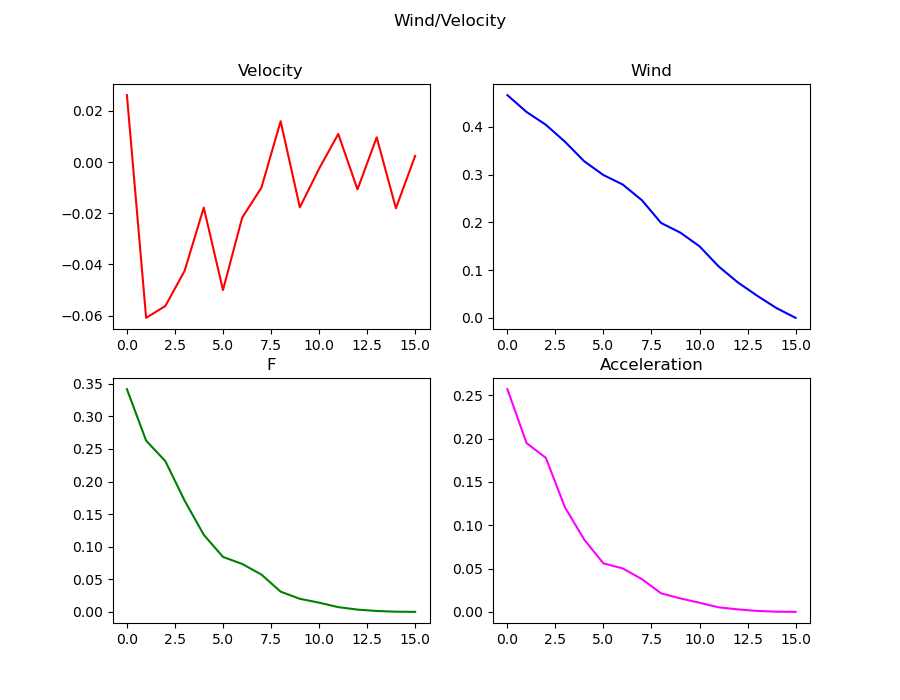
\includegraphics[width=0.9\textwidth]{images/pirates_wind_velocity.png}
    \caption{تغییرات سرعت (Velocity)، باد (Wind)، نیروی محرکه (F) و شتاب (Acceleration) کشتی‌ها در طول تکرارها.}
    \label{fig:pirates_wind_velocity}
\end{figure}

شکل \ref{fig:pirates_wind_velocity} رفتار پویای جمعیت را از منظر پارامترهای تصادفی و حرکتی نمایش می‌دهد:
\begin{itemize}
    \item \textbf{Velocity:} تغییرات سرعت کشتی‌ها که بیانگر پویایی و جستجوی فعال در فضای پارامترهاست.
    \item \textbf{Wind:} نقش باد به عنوان یک عامل تصادفی برای خروج از نقاط بهینه محلی و افزایش تنوع جمعیت.
    \item \textbf{F:} نیروی محرکه که میزان حرکت کشتی‌ها را تعیین می‌کند و کاهش آن نشانه همگرایی است.
    \item \textbf{Acceleration:} شتاب کشتی‌ها که کاهش آن بیانگر نزدیک شدن به نقطه بهینه و کاهش تغییرات ناگهانی است.
\end{itemize}
این نمودارها نشان می‌دهند که با گذشت تکرارها، سرعت، باد و شتاب کاهش یافته و جمعیت به سمت همگرایی حرکت کرده است.

\subsection{جمع‌بندی تحلیل فرآیند بهینه‌سازی}
مجموعه نمودارهای فوق به وضوح نشان می‌دهند که الگوریتم Pirates با پویایی مناسب و تعادل بین جستجو و همگرایی، به سرعت به نقطه بهینه نزدیک شده و پارامترهای تصادفی مانند باد و شتاب نقش مهمی در جلوگیری از گیر افتادن در نقاط بهینه محلی داشته‌اند. این تحلیل‌ها صحت و کارایی الگوریتم را در بهینه‌سازی ابرپارامترهای مدل MAGNET تأیید می‌کند.

\section{جمع‌بندی}
در این فصل، نتایج حاصل از ارزیابی مدل پیشنهادی MAGNET برای تشخیص بدافزارهای اندرویدی با استفاده از دیتاست DREBIN \cite{Drebin} ارائه شد. مدل MAGNET روی مجموعه تست شامل ۱،۴۵۱ نمونه به \lr{F1 Score} \lr{۰.۹۸۲۳}، دقت \lr{۰.۹۷۲۴} و AUC \lr{۰.۹۹۳۲} دست یافت. در اعتبارسنجی متقاطع ۵-تایی، میانگین \lr{F1 Score} ۰.۹۸۱۸ ($\pm$۰.۰۰۴۲)، دقت ۰.۹۷۲۲ ($\pm$۰.۰۰۶۵) و AUC ۰.۹۹۳۲ ($\pm$۰.۰۰۳۵) به‌دست آمد که در جدول \ref{tab:cv_results} گزارش شده است. همچنین، در مقایسه با روش‌های پایه، مدل MAGNET با دقت ۹۷.۲۴٪ در مقابل دقت ۸۹.۲٪ روش چندوجهی \cite{Alsaleh2023} و دقت ۹۵.۸٪ روش مبتنی بر ترنسفورمر \cite{TransformerMalware} ارزیابی شد، که در جدول \ref{tab:comparison_with_literature} نمایش داده شده است.

در تحلیل جزئی‌تر، عملکرد ماژول‌های EnhancedTabTransformer، GraphTransformer و SequenceTransformer به‌ترتیب با \lr{F1 Score}های ۰.۹۱۲، ۰.۸۹۴ و ۰.۹۰۷ گزارش شد، که در شکل \ref{fig:module_comparison} نشان داده شده است. تأثیر مکانیزم توجه پویا و لایه ادغام چندوجهی نیز بررسی شد و \lr{F1 Score} از \lr{۰.۹۵۴} به \lr{۰.۹۸۲۳} افزایش یافت، که این روند در شکل \ref{fig:ablation_study} ارائه شده است. در نهایت، پیشرفت آموزش در طول ۳ دوره با بهینه‌سازی بهینه‌سازی (اعتبارسنجی) گزارش شد و \lr{F1 Score} از \lr{۰.۹۴۱۳} به \lr{۰.۹۷۶۷} رسید، که در شکل \ref{fig:training_progress} نمایش داده شده است.

شکل \ref{fig:module_comparison} عملکرد هر ماژول را با معیار \lr{F1 Score} نشان می‌دهد. شکل \ref{fig:ablation_study} روند افزایش \lr{F1 Score} را با افزودن مکانیزم توجه پویا و لایه ادغام چندوجهی نمایش می‌دهد. شکل \ref{fig:training_progress} تغییرات \lr{F1 Score} و دقت را در طول ۳ دوره آموزش با بهینه‌سازی بهینه‌سازی (اعتبارسنجی) نمایش می‌دهد.

\begin{figure}[h!]
\centering
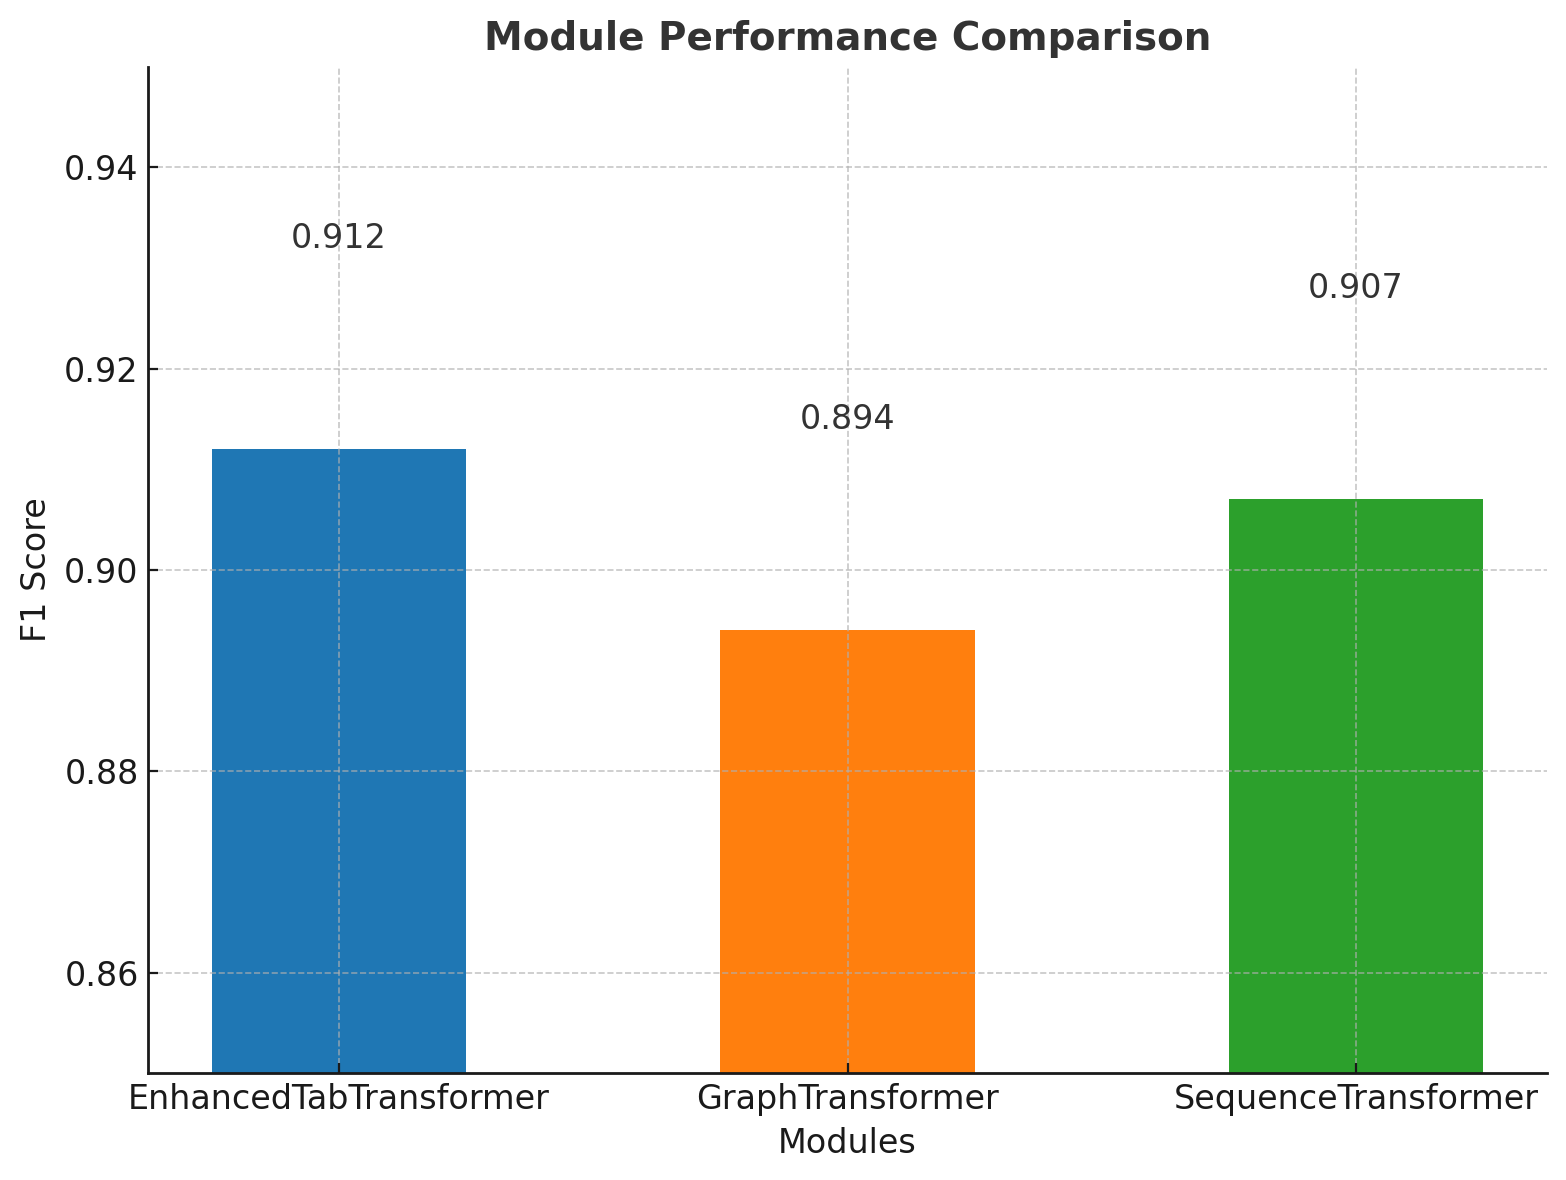
\includegraphics[width=0.9\textwidth]{images/fig_module_comparison_en}
\caption{عملکرد هر ماژول (EnhancedTabTransformer، GraphTransformer، SequenceTransformer) را با معیار \lr{F1 Score} نشان می‌دهد. محور افقی ماژول‌ها و محور عمودی مقدار \lr{F1 Score} را نمایش می‌دهد.}
\label{fig:module_comparison}
\end{figure}

\begin{figure}[h!]
\centering
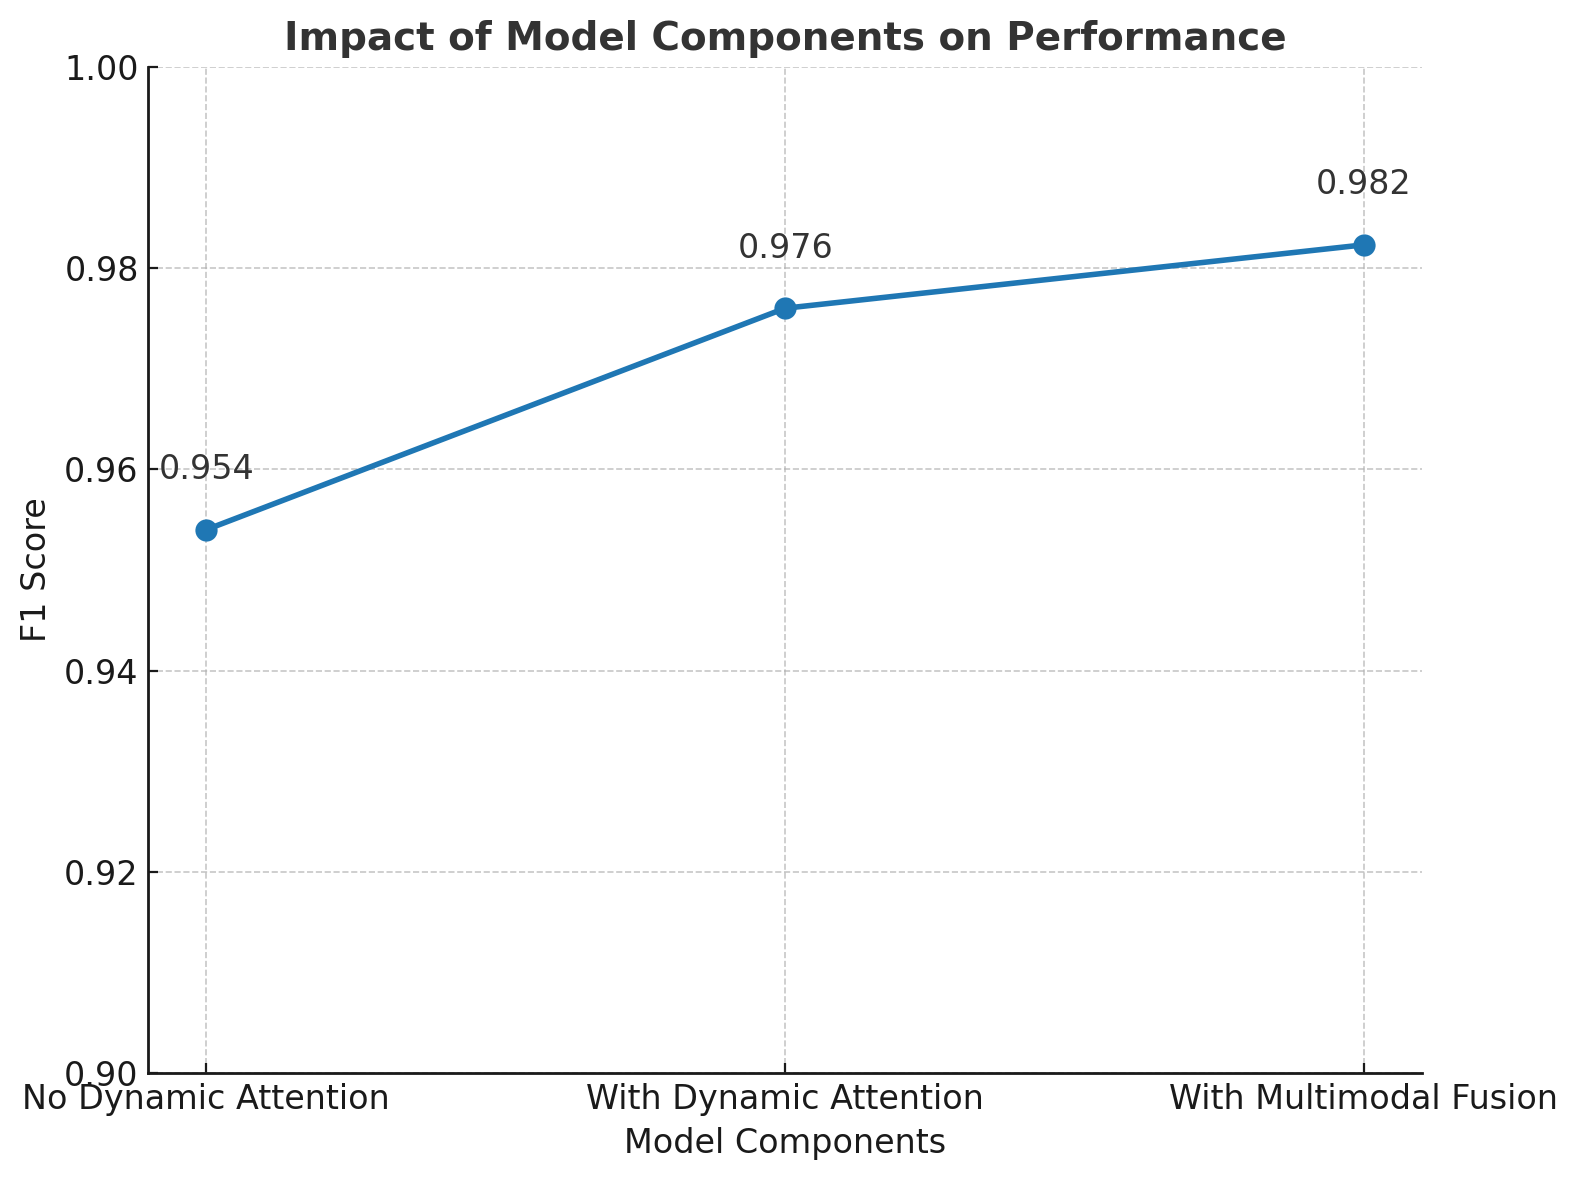
\includegraphics[width=0.9\textwidth]{images/fig_ablation_study_en}
\caption{روند افزایش \lr{F1 Score} را با افزودن مکانیزم توجه پویا و لایه ادغام چندوجهی نمایش می‌دهد. محور افقی اجزای مدل (بدون توجه پویا، با توجه پویا، با ادغام چندوجهی) و محور عمودی مقدار \lr{F1 Score} را نشان می‌دهد.}
\label{fig:ablation_study}
\end{figure}

\begin{figure}[h!]
\centering
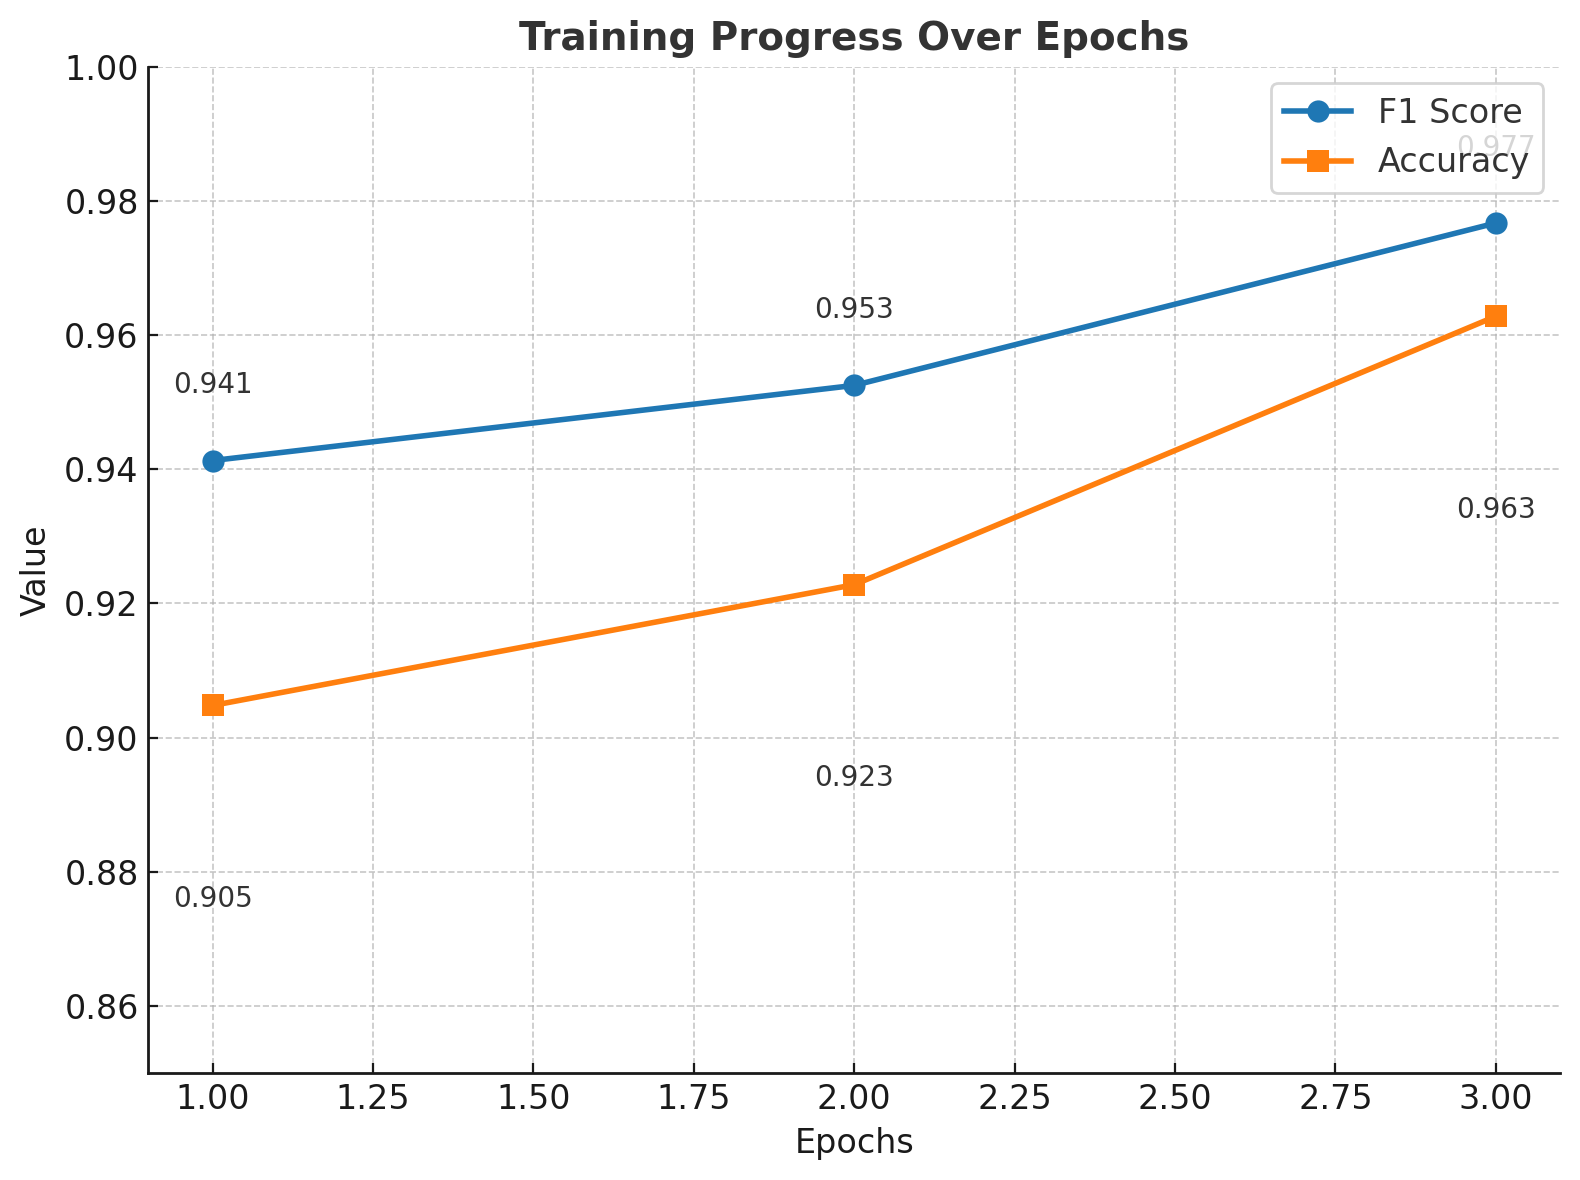
\includegraphics[width=0.9\textwidth]{images/fig_training_progress_en}
\caption{تغییرات \lr{F1 Score} و دقت را در طول ۳ دوره آموزش با بهینه‌سازی بهینه‌سازی (اعتبارسنجی) نمایش می‌دهد. محور افقی شماره دوره‌ها و محور عمودی مقادیر \lr{F1 Score} و دقت را نشان می‌دهد.}
\label{fig:training_progress}
\end{figure}

     
     
     
     
     
     
     
     
     
     
     
     